% -*-latex-*-

%% This is an example first chapter.  You should put chapter/appendix that you
%% write into a separate file, and add a line \include{yourfilename} to
%% main.tex, where `yourfilename.tex' is the name of the chapter/appendix file.
%% You can process specific files by typing their names in at the
%% \files=
%% prompt when you run the file main.tex through LaTeX.

% Beamline: Beam Energy
% BCM : charge
% BPM & raster:  beam position
% HRS Magenets: HRS Central momentum
% Scintillator & Trigger: livetime

\chapter{Experiment Setup}
\label{Experiement_Setup}

During an experiment that ran from October 10th  2007 to January 16th 2008, in Hall A of Thomas Jefferson National
Accelerator Facility (Jefferson Lab), the Coulomb Sum Rule was tested. To determine Coulomb Sum Rule, both response function $R_L$ and $R_T$ of different nuclei (${}^1$H, ${}^4$He, ${}^{12}$C, ${}^{56}$Fe, ${}^{208}$Pb) have been measured from inclusive scattering in the quasi-elastic region. In this chapter, the experiment setup and most of instrumentations will be introduced briefly. 

\section{Overview}

During the CSR experiment, an unpolarized electron beam was scattered from ${}^4$He, ${}^{12}$C, ${}^{56}$Fe and
${}^{208}$Pb target to measure the cross-section in quasi-elastic region. The Hall A High Resolution Spectrometer (HRS)
was used to detect the scattered electrons at 4 different angles: \SI{15}{\degree}, \SI{60}{\degree}, \SI{90}{\degree} and \SI{120}{\degree}.
The relative big difference between scattering angles allowed for the largest Rosenbluth lever arm within a single experiment compared to all previous experiments.
The cross section data were used to extract the $R_L$ and $R_T$ response functions and Coulomb Sum Rule.

To have as much covarage as possible in ($q$, $\omega$) to reduce systematic uncertainties in the Rosenbluth interpolation procedure,
the data were acquired in beam energies between 400 MeV and 3679 MeV , spectrometer central momentum between 100 MeV/$c$ and
3.6 GeV/$c$, see Table.~\ref{tab:E_E'_table}. The kinematic coverage of the CSR experiment is shown in Figure.~\ref{fig:kinematic_coverage}.

\begin{table}[tb!]
\center
\begin{tabular}{|c|c|c|c|c|c|c|c|}
\hline
\multicolumn{2}{|c|}{\SI{15}{\degree}} & \multicolumn{2}{c|}{\SI{60}{\degree}} & \multicolumn{2}{c|}{\SI{90}{\degree}} & \multicolumn{2}{c|}{\SI{120}{\degree}} \\ \hline
$E$      & $E'_{low}$    & $E$     & $E'_{low}$    & $E$     & $E'_{low}$    & $E$     & $E'_{low}$     \\ \hline
1260     & 810           & 646     & 187           & 400     & 100           & 400     & 100            \\
1646     & 1147          & 740     & 250           & 528     & 108           & 528     & 98             \\
2145     & 1605          & 845     & 305           & 646     & 127           & 646     & 107            \\
2448     & 1838          & 957     & 377           & 740     & 170           & 740     & 110            \\
2845     & 2135          & 1030    & 270           & 845     & 135           & 845     & 105            \\
3249     & 2440          & 1102    & 333           & 957     & 267           & 957     & 237            \\
3679     & 2770          & 1260    & 370           & 1030    & 100           &         &                \\ \hline
\end{tabular}
\caption[E E' talbe]{Incident energy and the lowest scattered energy detected (in MeV) at each kinematics.} \label{tab:E_E'_table}
\end{table}

\begin{figure}[h]
\centering
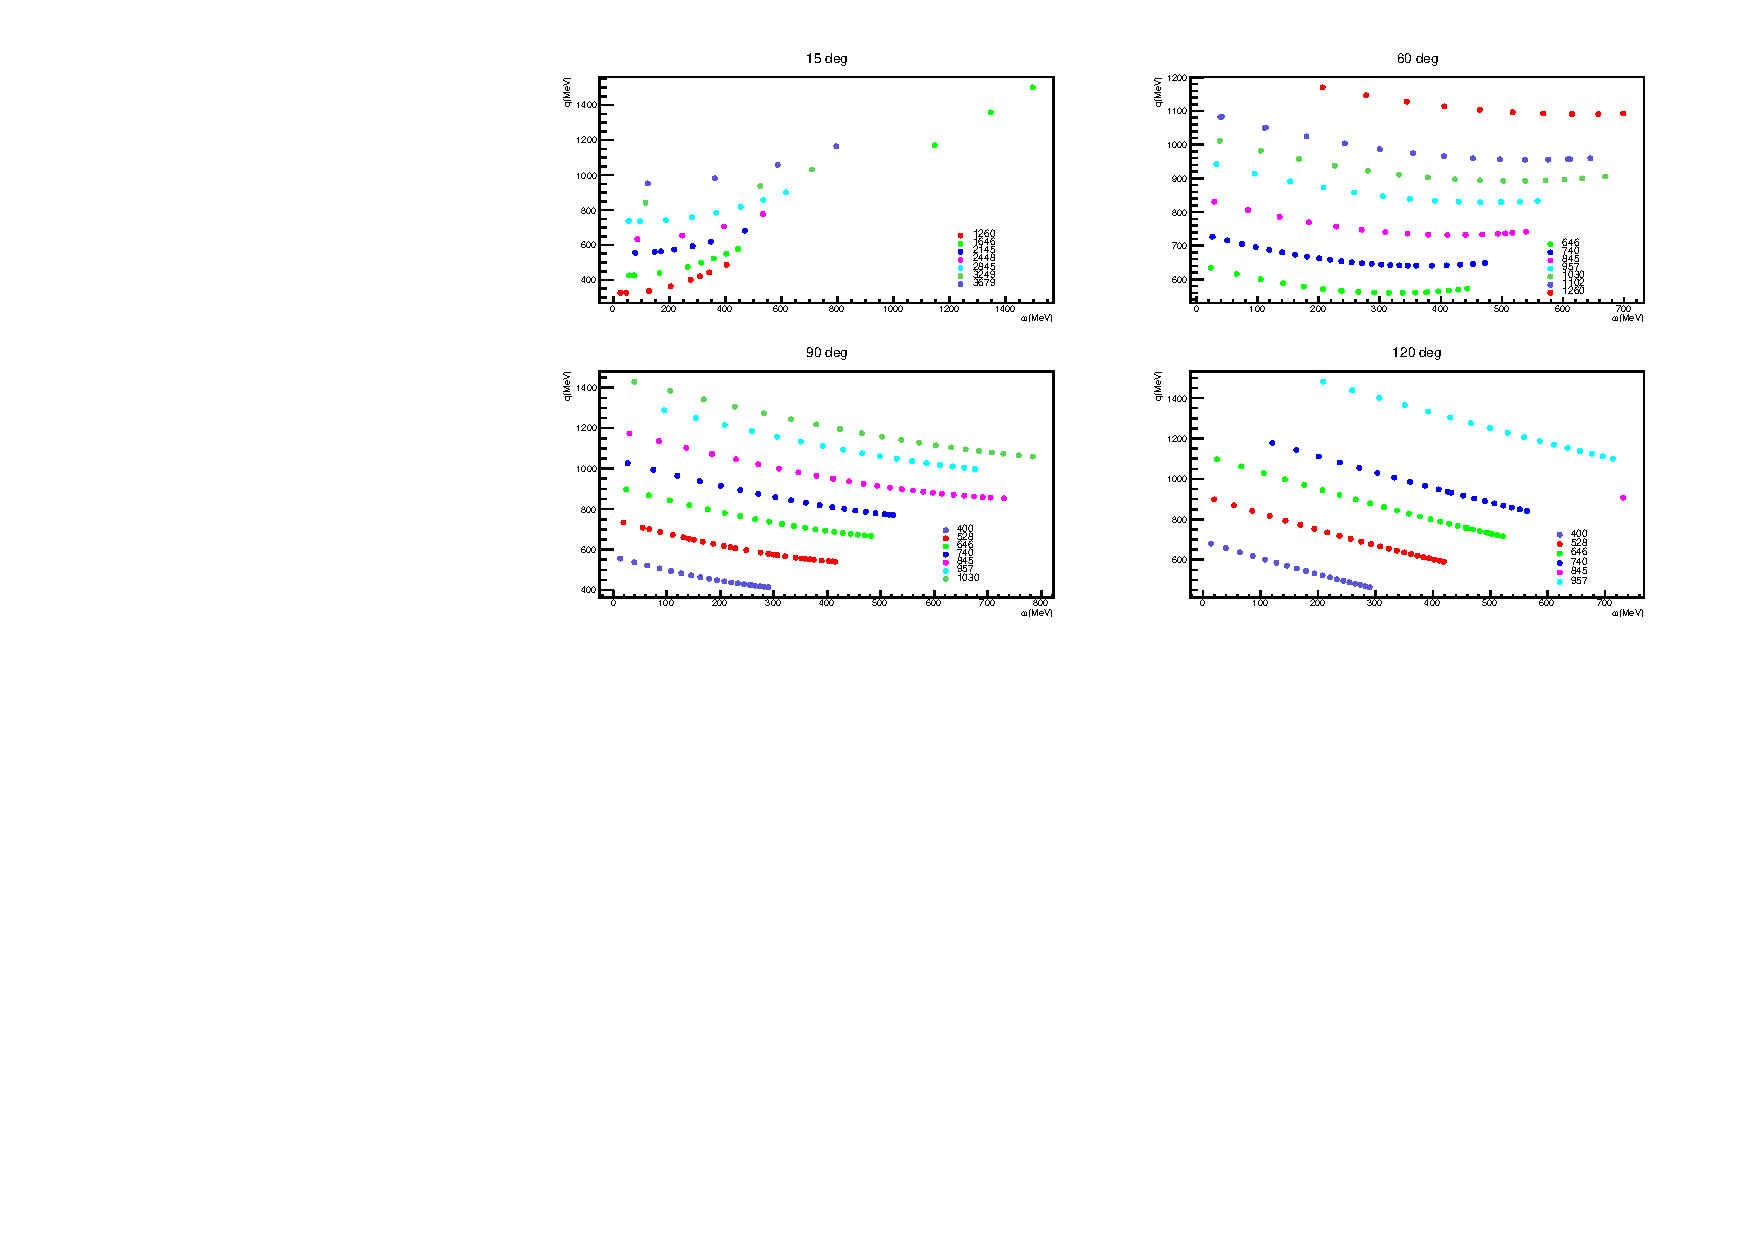
\includegraphics[width=0.7\textwidth]{figs/He4kinematics.pdf}
\caption[He4 kinematic]{Kinematic coverage of the CSR experiment. Each graph for a scattering angle, each color represent a beam energy.
The y axis is three momentum transfer (MeV) and the x axis is energy loss $\omega$ (MeV).
\label{fig:kinematic_coverage}}
\end{figure}

This chapter will discuss the electron beam, the Hall A beamline components, the cryogenic and solid targets and the HRS system.

\section{The Accelerator and Electron Beam}
The Continuous Electron Beam Accelerator Facility (CEBAF) at Jefferson Lab (JLab) was built to investigate the structure
of nuclei and hadrons and the underlying fundamental interactions in the region below the high-energy "asymptotically
free" regime. 

The accelerator consists of an electron injector, two super-conducting linear accelerators, recirculation arcs,
and RF separators. The layout of accelerator is shown in Figure.~\ref{fig:JLab_overview}.


\begin{figure}[h]
\centering
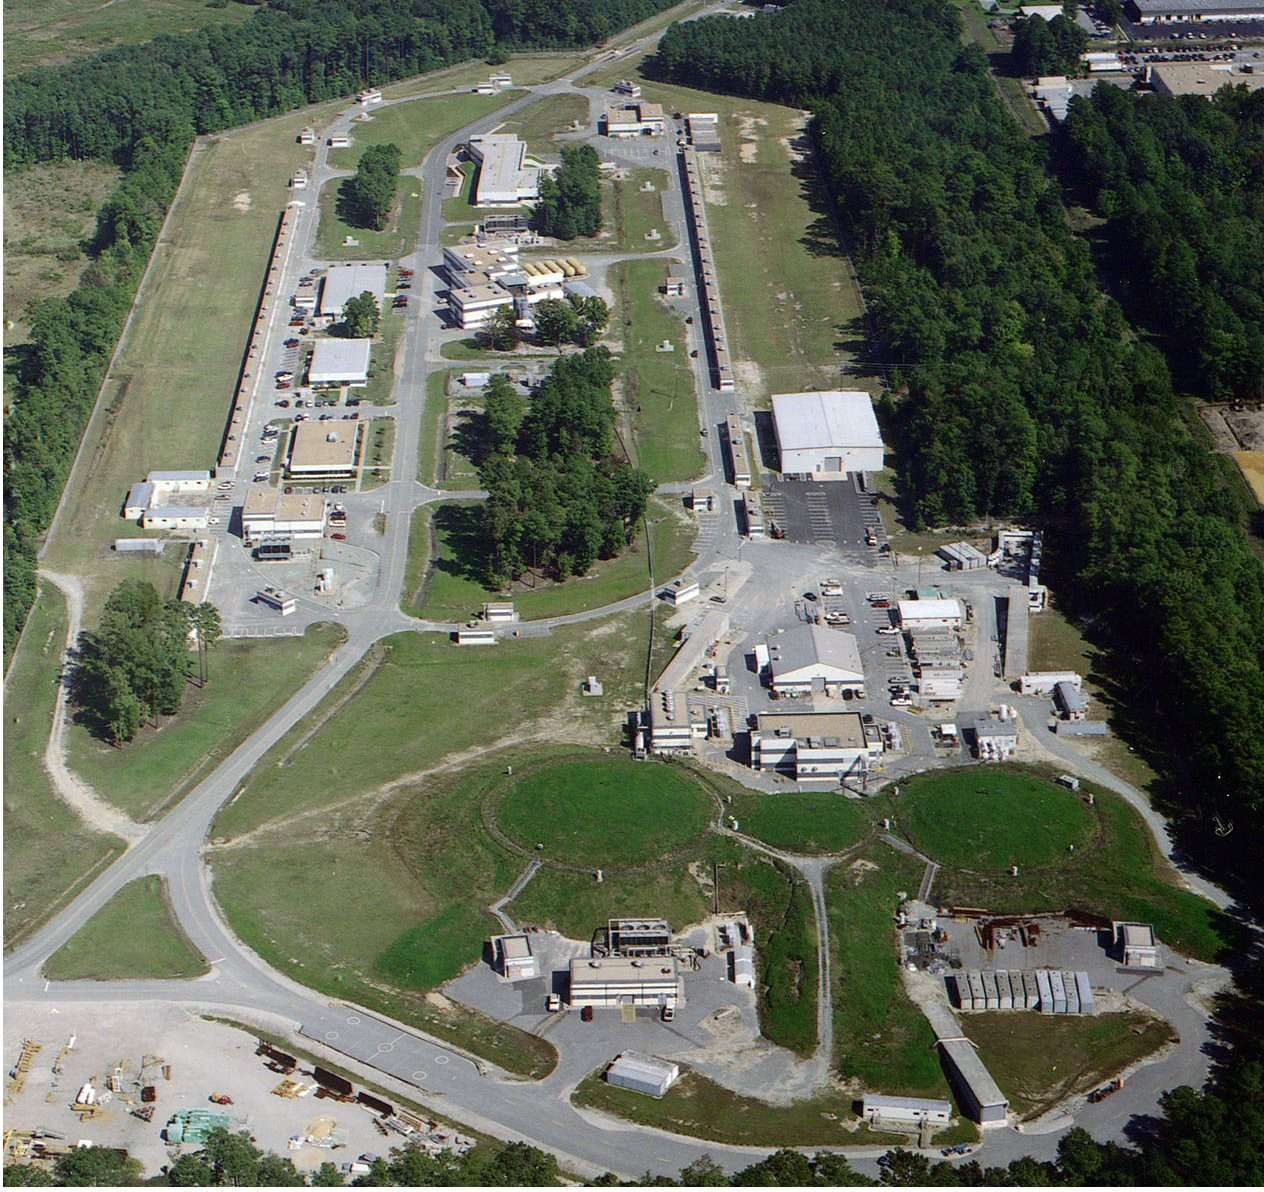
\includegraphics[width=0.7\textwidth]{figs/JLab_overview.png}
\caption[JLab overview]{JLab overview.  \label{fig:JLab_overview}}
\end{figure}

%injector
The source of polarization electrons is a strained GaAs cathode at injector. The cathode is illuminated by a 1497 MHz
gain-switched 780 nm diode laser.  It provides polarized beam of above 70\% polarization.

% linacs
The beam is first accelerated to 45 MeV in the injector, then is transported to the north linac. Each linac
contains 20 cryomodules (this was the situation before 12 GeV upgrade; 5 new cryomodules were added to each linac after the
upgrade). There are eight super-conducting niobium RF cavities in each cryomodule. The RF cavities are phased to provide
maximum acceleration. The nominal gain of each linac is 400 MeV, and it can be tuned up to 500 MeV, which made it possible to accelerate the beam up to 5.7 GeV.
Liquid Helium from the at CHL (Central Helium Liquefier) keeps the superconducting cavities at a temperature of 2 K.

%arcs
The north and the south linacs are connected by recirculation arcs with radius 80 m that can turn the beam by
\SI{180}{\degree} from the south to the north linac and vice versa, forming a recycling beamline in the shape
of a "racetrack". Each arc has more than 2,200 quadruple or dipole magnets to provide the field that keeps the beam on a precise
path and tightly focused.

After passing through the south linac, the beam can either go to the next recirculation arc for another pass around the accelerator, or enter one of the
experiment halls using RF extraction. The designed maximum current is 200 $\mu$A, which can be split arbitrarily to
three 499 MHz bunch trains, one for each hall.  The CSR experiment required 50 $\mu$A average current, with energies ranging from 0.4 to 4 GeV.


\section{Beam Energy Measurement}
There beam energy measurement is an important part of the experiment to ensure the accuracy. There are two independent
methods to measure the absolute beam energy :  Arc measurement, which is based on measurements of the beam deflection in
a known field; and eP measurement, which is based on measurement of the electron elastic scattering off carbon target.  
During the CSR experiment, only the Arc measurement was used.

%% Measurement principle; uncertainty; 
\subsection{Arc Measurement}
The principle of this method is that electrons in a magnetic field will move in circular patten, with the radius
depending on field strength and electron's momentum. The Arc method measures the bending radius of the beam in the
arc section, see Figure.~\ref{fig:arc-measurement}. 

\begin{figure}[tb!]
\centering
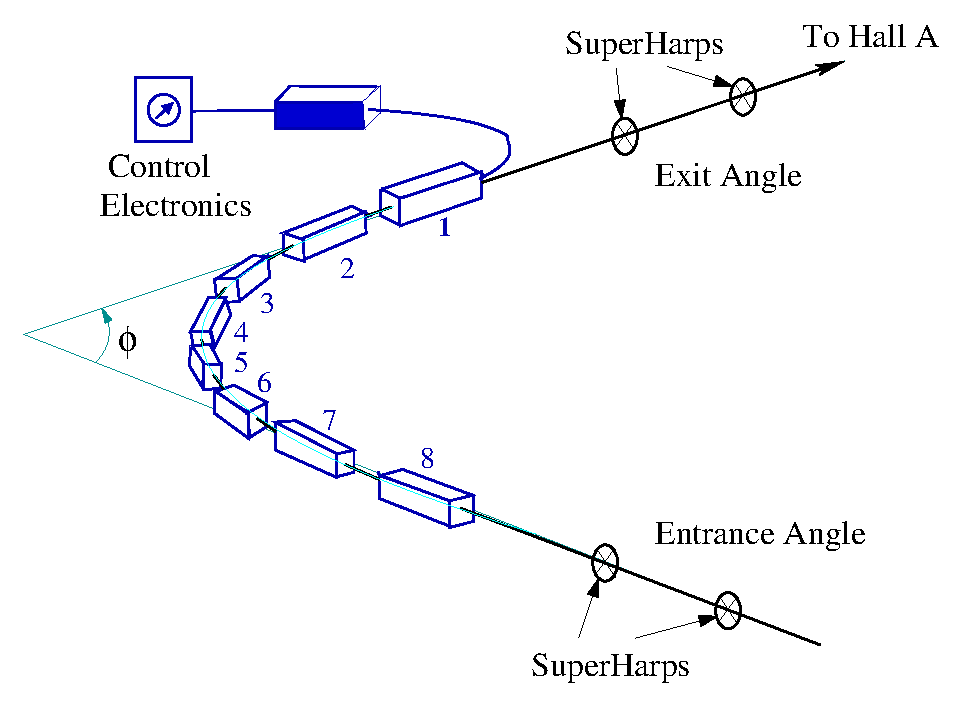
\includegraphics[width=0.8\textwidth]{figs/arc-measurement.pdf}
\caption[Arc Measurement]{Arc section of Hall A beamline.  \label{fig:arc-measurement}}
\end{figure}

The momentum of the beam ($p$ in GeV/c) is then related to the field integral in eight dipoles ($\int\vec{B}\times\partial\vec{l}$
in T$\cdot$ m) and the net bending angle through the arc section ($\theta$ in radians) by:
\begin{equation}
  P = k \frac{\int\vec{B}\times\partial\vec{l}}{\theta}
\end{equation}

where $k=0.299792$ GeV $\cdot$ rad $\cdot$ T$^{-1}$ $\cdot$ m $^{-1}$. 

Detailed description of the Arc measurement can be found in \cite{Alcorn2004}.
The arc measurement consists of two simultaneous measurements. One is for the bending angle of the beam measured by a set of wire scanners. Another is for the field strength integral $\int\vec{B}\times\partial\vec{l}$ of the eight dipoles based on the reference magnet(9 th dipole) field measurement.
There are two operation modes in the arc section: the dipersive (invasive) and non-dispersive(non-invasive) mode. The
dispersive mode will affect the quality of the beam, but has better precision ($\Delta E_{beam}/E_{beam} = 2\times10^{-4}$) than non-dispersive mode ($5\times10^{-4}$).

The Arc measurement during the CSR experiment is done at a beam energy of 845 MeV. The measurement result ($845.08 \pm
0.2$ MeV) is consistent with the so-called "Tiefenbach" energy ($844.87 \pm 0.4$ MeV), calculated from the Hall A arc
$\vec{B}\partial\vec{l}$ value and the Hall A beam position measured from the beam position monitor(BPM). 

%The uncertainty of the Arc measurement is at $2\times10^{-4}$ level.

%\section{Hall A Overview}
%The Hall A has a diameter of 53 m. The basic layout of Hall A is shown in figure below. It basically can be divided into three parts: the beamline appratus (BPM, BCM, Raster, Moller, Compton, etc), target system, the left and right HRS spectrometers(??).

%\begin{figure}
%\centering
%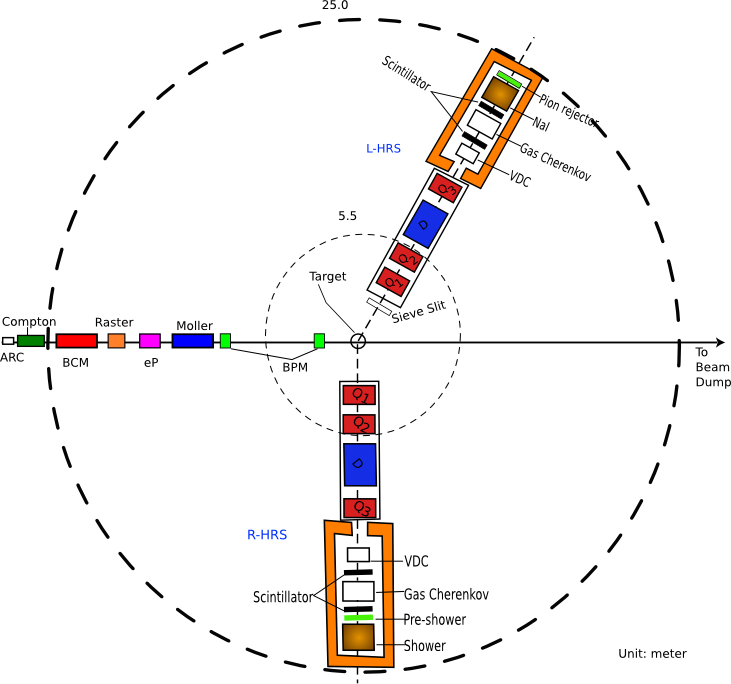
\includegraphics[width=\textwidth]{figs/Hall_A_overview.png}
%\caption[Hall A Overview]{Hall A Overview.  \label{Hall_A_overview}}
%\end{figure}


\section{Beam Charge Measurement}
The incident number of beam electrons is an essential normalization factor in the extraction of cross sections.
It is proportional to the beam current measured by the Beam Current Monitor (BCM) in Hall A,
which provides a stable, low-noise, non-interfering beam current measurement \cite{Alcorn2004}.

The BCM consists of an Unser monitor, two RF cavities, associated electronics and a data-acquisition system.
The diagram of BCM is shown in Figure.~\ref{fig:BCM_diagram}.
The cavities and the Unser monitor are located 25 m upstream of the target.
The Unser monitor is a parametric current monitor which provides an absolute reference.  
The two resonant FR cavity monitors on two sides on the Unser Monitor are stainless steel
cylindrical high-Q ($~$ 3000) waveguides which are tuned to the frequency of the beam (1.497 GHz)
resulting in voltage levels at their outputs being proportional to the beam current.
Each of the RF output signals from the two cavities is split into sampled and integrated parts.

\begin{figure}[tb!]
\centering
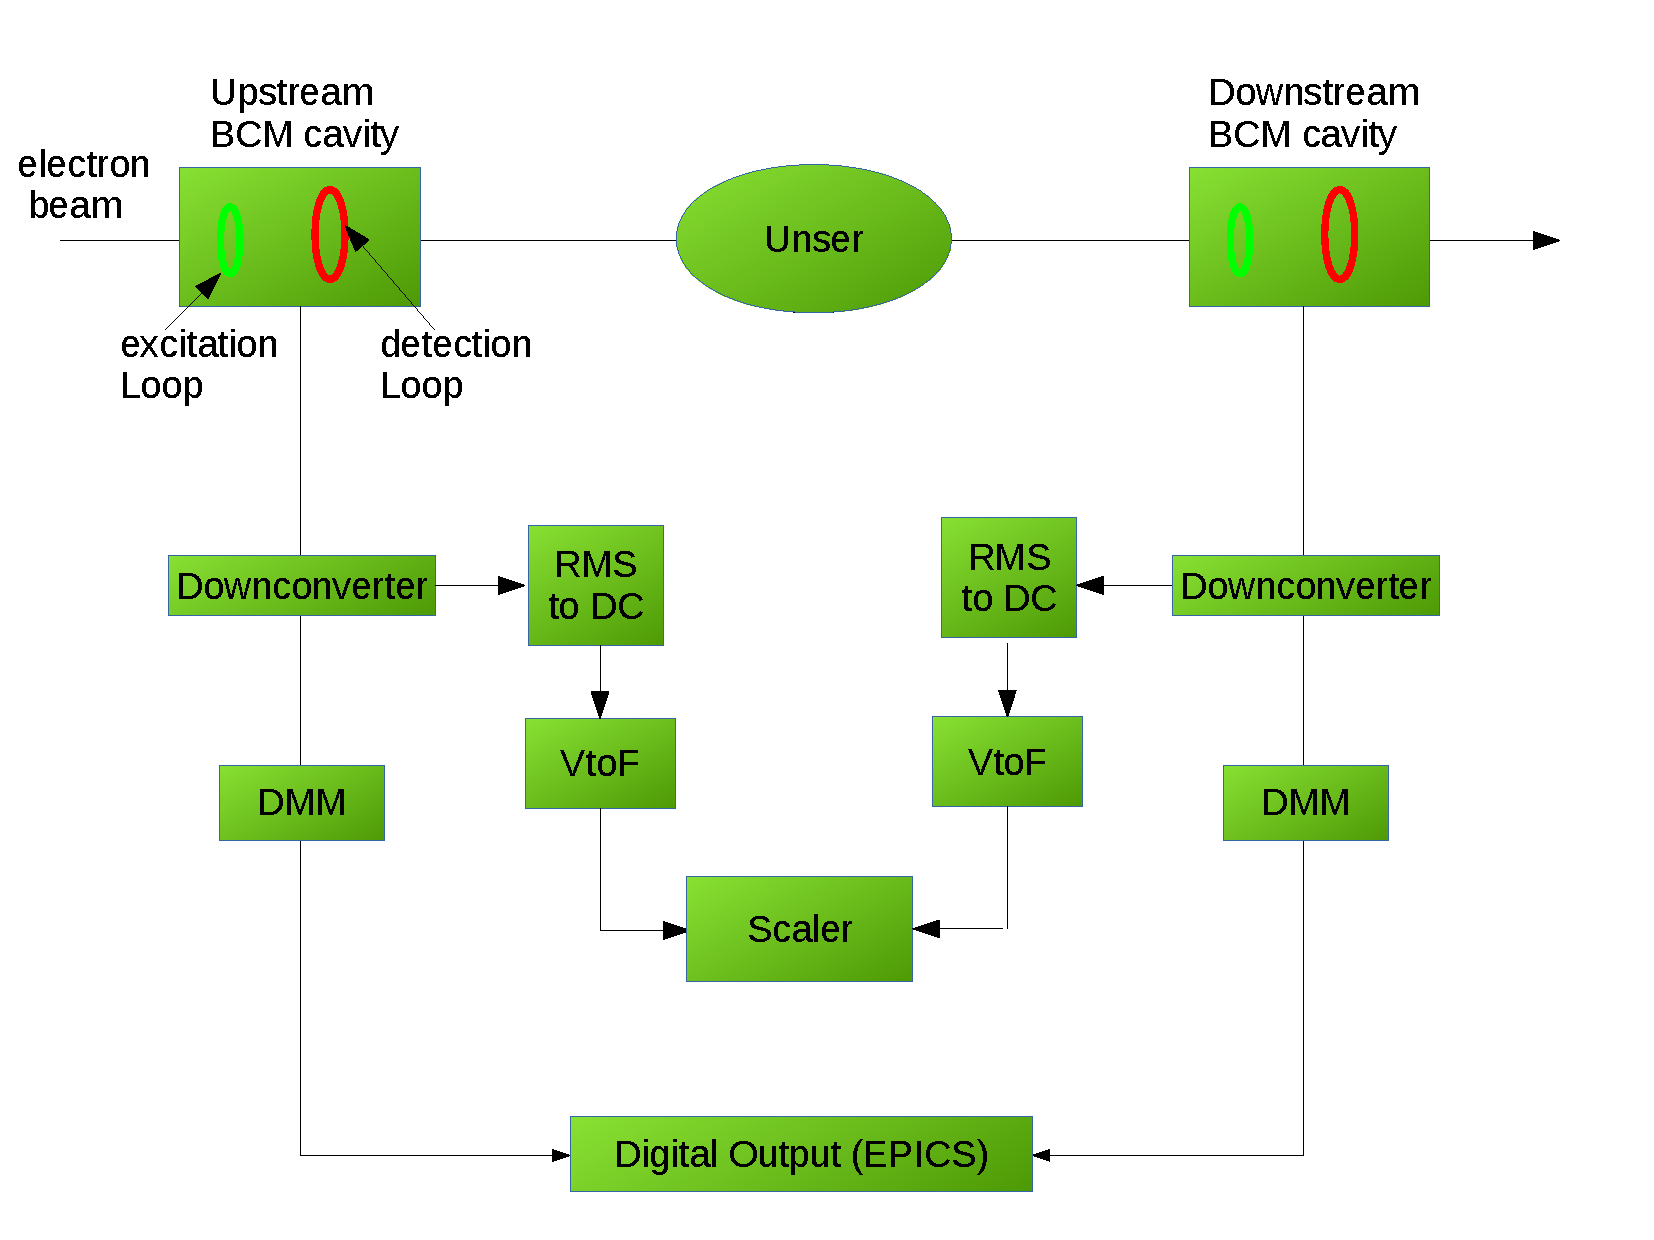
\includegraphics[width=0.8\textwidth]{figs/BCM_diagram.pdf}
\caption[BCM diagram]{Beam current monitor diagram. Plot reproduced from \cite{Alcorn2004}.   \label{fig:BCM_diagram}}
\end{figure}


The sampled data is sent to a high-precision Digital Multi-Meter (DMM),
which provides an output signal representing the RMS of the input signal
during that second. The output is proportional to the beam charge accumulated
for that second. The signals from both cavities are sent to a computer
through GPIB cables, and are recorded every 1-2 s in the EPICS 
(Experimental Physics and Industrial Control System) database.

The integrated data is sent to an RMS-to-DC converter to generate
an analog DC voltage level. The voltage level is sent to 
a Voltage-To-Frequency(VtoF) converter whose output frequency is
proportional to the input.
The frequency signal is fed to 200 MHz VME scalers and stored in
stream with other scaler information every 4 seconds.
The scaler value accumulates during the run and is proportional
to the time-integrated voltage level.
The regular RMS to DC output is linear for currents from 5$\mu A$ to
200 $\mu A$. A set of amplifiers with different gain factors ($\times$ 1,
$\times$ 3, $\times$ 10) can extend the linear region to lower currents.
%So there are three signals from each RF cavity (U1, U3, U10 or D1, D3 D10). 
The six signals for each spectrometer (U1, U3, U10 and D1, D3, D10, corresponding to the 3 gain factors and the up and
downstream cavities respectively) are sent to scalers and provide
the charge information during a run with redundancy.

The beam charge can be derived from BCM scaler reading as
\begin{equation}
Q_{bcm \times n} (\mu C) = \frac{\frac{Scaler_{bcm \times n}}{T} -Offset_{bcm \times n}}{Constant_{bcm \times n}} T
\end{equation}
where n=1, 3, 10 is the gain factor of the amplifiers, $T$ is the clock time for each run (in seconds),
Scaler$_{bcm \times n}$ is the BCM scaler reading for each gain factor.
The Offset$_{bcm \times n}$ and Constant$_{bcm \times n}$ are calibrated in BCM calibrations during CSR experiment, and are
given in Table ~\ref{tab:BCM_calibration}.

%The BCM calibration during CSR experiment gave the values of scaler calibration constants and offsets of upstream and
%downstream cavities, which are listed in Table .\ref{tab:BCM_calibration}.

\begin{table}[tb!]
\centering
\begin{tabular}{|c|c|c|c|c|}
\hline
Gain & \begin{tabular}[c]{@{}c@{}}Upstream\\ Calibration Constants\end{tabular} & \begin{tabular}[c]{@{}c@{}}Upstream\\
Offsets\end{tabular} & \begin{tabular}[c]{@{}c@{}}Downstream\\ Calibration Constants\end{tabular} &
\begin{tabular}[c]{@{}c@{}}Downstream\\ Offsets\end{tabular} \\ \hline
1    & 2372.38                                                                  & 362.5
& 24727.91                                                                   & 160.1
\\ \hline
3    & 7294.51                                                                  & 350.2
& 7517.37                                                                    & 126.7
\\ \hline
10   & 22067.11                                                                 & 442.6
& 23485.15                                                                   & 321.1
\\ \hline
\end{tabular}
\caption[BCM calibration]{BCM calibration constants and offsets.} \label{tab:BCM_calibration}
\end{table}

\section{Beam Position Monitor and Raster}
The beam typically has a Gaussian distribution across the cross-sectional area with full width at half maximum (FWHM)
$\sigma \approx$ 100 $\mu$m. To avoid damaging the target, the beam is rastered to a few millimeters in size. 
The raster is a pair of horizontal (X) and vertical (Y) air-core dipoles located 23 m upstream of the target.
There are two modes of the raster: sinusoidal and amplitude modulated.
In the sinusoidal mode, both X and Y dipoles are driven at 18 kHz with a \SI{90}{\degree} phase difference
which produces a circular pattern. The radius of the circular pattern is controlled by a function generator.
In the CSR experiment, a 2 mm $\times$ 2 mm sinusoidal mode was used on both the cryogenic targets and solid targets.

The beam position is an important parameter for the optics calibration and acceptance calculation of the spectrometers.
Two Beam Position Monitors located at 7.524 m and 1.286 m upstream of the target are used to determine the 
 position and direction of the beam at the target. 
Each BPM consists of four wire antennas parallel to the beam direction, which are tuned to the beam RF frequency 1.497 GHz.
They are placed symmetrically around the beam pipe in a vacuum chamber.
When a electron passes through the BPM, it will induce signals in antennas.
The amplitude of signal in each antenna is reverse by proportional to the distance between the antenna and the beam.
%So the beam position can be extracted in the BPM local coordinates.

The absolute position of the BPMs can be calibrated with respect to the harps near each of the BPMs.
The beam position information are stored in two ways:

\begin{enumerate}
\item The average beam position data over a 0.3 s time period are recorded in EPICS database and injected asynchronously
into the data stream
every 3-4 s.
\item The event-by-event beam position information is recorded in the CODA data stream from each of the 8 BPM antennas (2
$\times$ 4), and are also recorded in the data stream.
\end{enumerate}

The beam position and direction can be reconstructed from BPM information $x_{bpma,b}$ and $y_{bpma,b}$ as:

\begin{equation}
x_{beam} = \frac{x_{bpma} \cdot z_{bpmb} - x_{bpmb} \cdot z_{bpma}}{z_{bpmb}-z_{bpma}}
\end{equation}

\begin{equation}
y_{beam} = \frac{y_{bpma} \cdot z_{bpmb} - y_{bpmb} \cdot z_{bpma}}{z_{bpmb}-z_{bpma}}
\end{equation}

\begin{equation}
\theta_{beam} = \frac{x_{bpmb} - x_{bpma} }{z_{bpmb}-z_{bpma}}
\end{equation}

\begin{equation}
\phi_{beam} = \frac{y_{bpmb} - y_{bpma} }{\sqrt{(x_{bpmb} - x_{bpma})^2+(z_{bpmb}-z_{bpma})^2 }}
\end{equation}
where $z_{bpma}$ = -7.345 m, $z_{bpmb}$ = -2.214 m.  


% target structure
% solid target, liquid target (LH, LHe)

\section{Target System}

\subsection{Target Chamber}
The standard target vacuum chamber is used in the CSR experiment (see Figure.~\ref{fig:target_chamber}). The vacuum chamber is constructed out of several 1037-mm diameter rings, supported on a 607-mm diameter central pivot post. 
The stainless-steel base ring has one vacuum pump-out port and other ports for viewing and electrical feed-throughs. The
middle ring is made out of aluminum and located at the beam
height with 152-mm vertical cutouts on each side of the beam over the full angular range (that can accommodate
scattering angles within \SI{12.5}{\degree} $\leq$ $\theta$
$\leq$\SI{167.5}{\degree}). The cutouts are covered with
a pair of flanges with thin (0.38 mm) aluminum foils. It also has entrance and exit beam ports. The upper ring is used to house the cryotarget.

\begin{figure}[tb!]
\centering
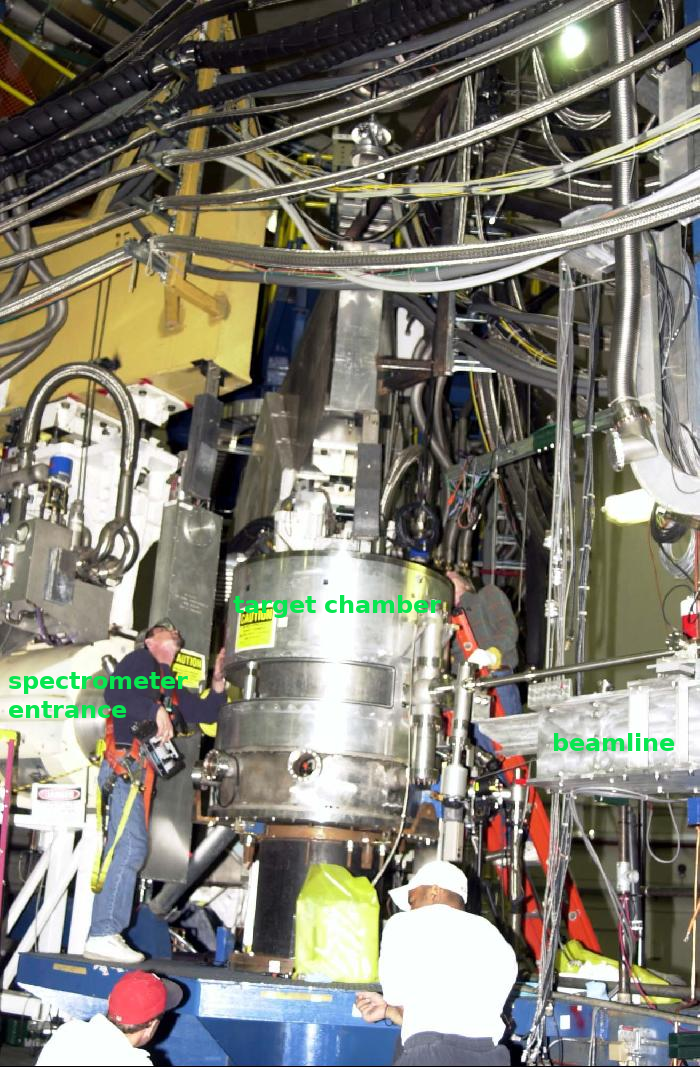
\includegraphics[width=0.6\textwidth]{figs/target_chamber_word.png}
\caption[Hall A target chamber]{Hall A target chamber.  \label{fig:target_chamber}}
\end{figure}

\subsection{Target Configuration of CSR}
The CSR experiment used targets from light nuclei to heavy nuclei in order to study medium dependency of 
Coulomb Sum rule.
Several targets: $^{2}$H, $^{4}$He, $^{12}$C, $^{23}$Al, Empty, BeO, $^{56}$Fe and $^{208}$Pb --- were used in this experiment.
These targets were installed on a target ladder in the target chamber and can be controlled remotely.


The position of the target ladder is vertical in the path of the electron beam.
The target system is controlled by three servo motors, each connected to its own motion controller called a BDS.
Two of  the BDS units are configured as "Slaves" and are controlled by the third, the "Master".
The target operator moves the target with the Master BDS through IOCs(input-output controllers) during the
experiment.
The various target positions are stored as 15 encoder values on the control computer (IOC). An encoder that is attached to
the Master's servo motor determines the target BDS position. The target positions are listed in Table~\ref{tab:tgmat-BDS}.

\begin{table}[tb!]
\centering
\begin{tabular}{lrr}
\hline
Target            & Material         & BDS Position \\ \hline
Loop 1 10cm       & High Pressure He & 32932800     \\
Loop 2 15 cm + Pb & He + Pb          & 26954176     \\
Loop 2 10 cm      & He               & 23377856     \\ \hline
Loop 3 15 cm + Pb & H$_2$ + Pb       & 19802560     \\
Loop 3 10 cm      & H$_2$            & 16241600     \\ \hline
Optics            & 7 carbon foils   & 12760000     \\
10 cm dummy       & 2 Al foils       & 10092480     \\
15 cm dummy       & 2 Al foils       & 9370560      \\
Empty             & N/A              & 8653760      \\
BeO               & BeO              & 6406480      \\
Beam right carbon & Carbon           & 4321550      \\
Beam right iron   & Iron             & 2692366      \\
Beam left carbon  & Carbon           & 585998       \\
Beam left iron    & Iron             & -1040625     \\ \hline
\end{tabular}
\caption[Target Materials and BDS Position.]{Target Materials and BDS Position for CSR experiment.}\label{tab:tgmat-BDS}
\end{table}

%cryogenic target
The cryogenic targets are mounted on the top layer of target ladder inside the target chamber with sub-system for cooling,
gas handling, temperature and pressure monitoring. 
The cryogenic target has three independent target loops, one gaseous helium loop (Loop 1) and two liquid hydrogen (LH2)
loops (Loop 2 and 3).

The Loop 1 target is a vertical "racetrack" shape cell, it is 10 cm long and 2cm wide. (See Figure.~\ref{fig:loop1})

\begin{figure}[tb!]
\centering
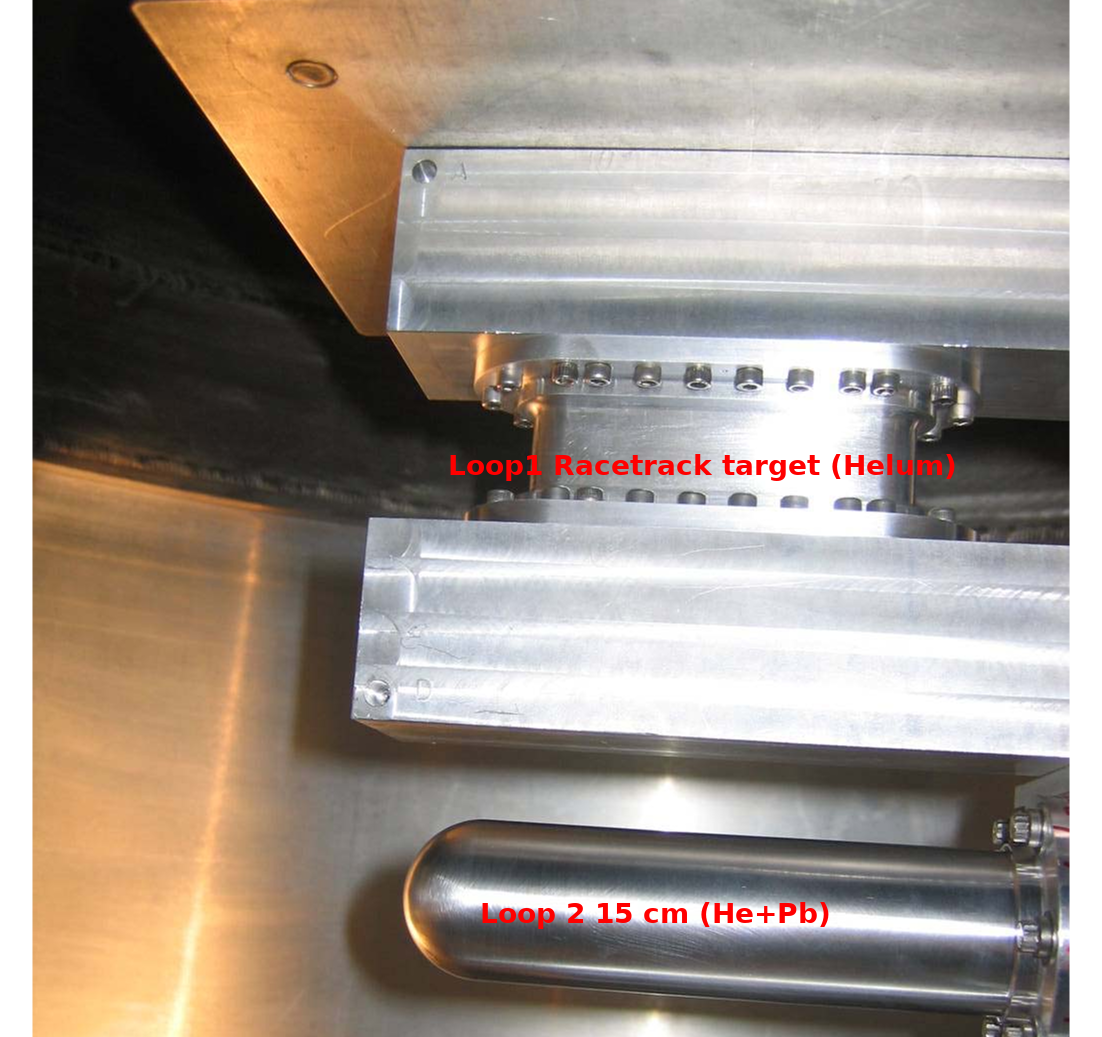
\includegraphics[width=0.8\textwidth]{figs/Loop1_target_edit.png}
\caption[Loop 1 cryogenic target ]{Loop 1 cryogenic target ($^4$He) }\label{fig:loop1}
\end{figure}

Loop 2 has two aluminum cylindrical target cells filled with Helium.
%comment: the 2 cells of Loop 2 both filled with Helium.
The upper cell is 15 cm long with a $^{208}$Pb foil held at the center
and tilted 50.0 $\pm$ \SI{2.00}{\degree} to the beam right, for cooling purpose.  The lower cell is 10 cm long filled
with $^{4}$He only.
Similarly, Loop 3 has 2 aluminum cylindrical target cells, both 15 cm long. The upper cell has a $^{208}$ Pb foil at
the center, also tilted 50.0 $\pm$ \SI{2.00}{\degree} to the beam right.
The lower cell is 15 cm long filled with liquid hydrogen only.
Loop 2 and Loop 3 cryogenic targets are shown in Figure.\ref{fig:loop2_loop3}.
Table.\ref{tab:window_thickness} gives the cell window and lead target thickness.

\begin{table}[tb!]
\centering
\scriptsize
\begin{tabular}{|l|l|l|r|l|l|}
\hline
Cryogenic Target & \begin{tabular}[c]{@{}l@{}}Entrance Window\\ (mm) $\pm$ 0.005\end{tabular} &
\begin{tabular}[c]{@{}l@{}}Exit Window\\ (mm) $\pm$ 0.005\end{tabular} & \begin{tabular}[c]{@{}r@{}}Lead thickness\\
($g/cm^2$)\end{tabular} & Beam left wall (mm) & Beam right wall (mm) \\ \hline
Loop1 10 cm      & 0.263 $\pm$ 0.008                                                          & 0.280 $\pm$ 0.005
& N/A                                                                 & 0.245 $\pm$ 0.002   & 0.239 $\pm$ 0.007    \\
\hline
Loop2 15 cm      & 0.128 $\pm$ 0.002                                                          & 0.194 $\pm$ 0.009
& 0.1057 $\pm$ 0.0001                                                 & 0.194 $\pm$ 0.009   & 0.194 $\pm$ 0.009    \\
\hline
Loop2 10 cm      & 0.257 $\pm$ 0.005                                                          & 0.120 $\pm$ 0.070
& N/A                                                                 & 0.120 $\pm$ 0.070   & 0.120 $\pm$ 0.070    \\
\hline
Loop3 15 cm      & 0.129 $\pm$ 0.001                                                          & 0.207 $\pm$ 0.005
& 0.3187 $\pm$ 0.0004                                                 & 0.207 $\pm$ 0.005   & 0.207 $\pm$ 0.005    \\
\hline
Loop3 15 cm      & 0.217 $\pm$ 0.003                                                          & 0.115 $\pm$ 0.001
& N/A                                                                 & 0.115 $\pm$ 0.001   & 0.115 $\pm$ 0.001    \\
\hline
\end{tabular}
\caption[Cryotargets window and lead target thicknesses]{Cryotargets window and lead target
thicknesses.}\label{tab:window_thickness}
\end{table}

The $^{4}$He gas target was operated at 7.0 K and about 170 psi, with a density about 0.12 g/cc. 
The nominal operating conditions of liquid targets are: 6.3 K at 1.4 MPa for $^{4}$He in Loop 2, 
and 19.0 K at 0.17 MPa for $^{2}$H in Loop 3.
The targets are cooled with helium supplied by the ESR (End Station Refrigerator).
The uncertainty in the target density is minimized by monitoring the pressure and temperature with pressure transducers.

\begin{figure}[tb!]
\centering
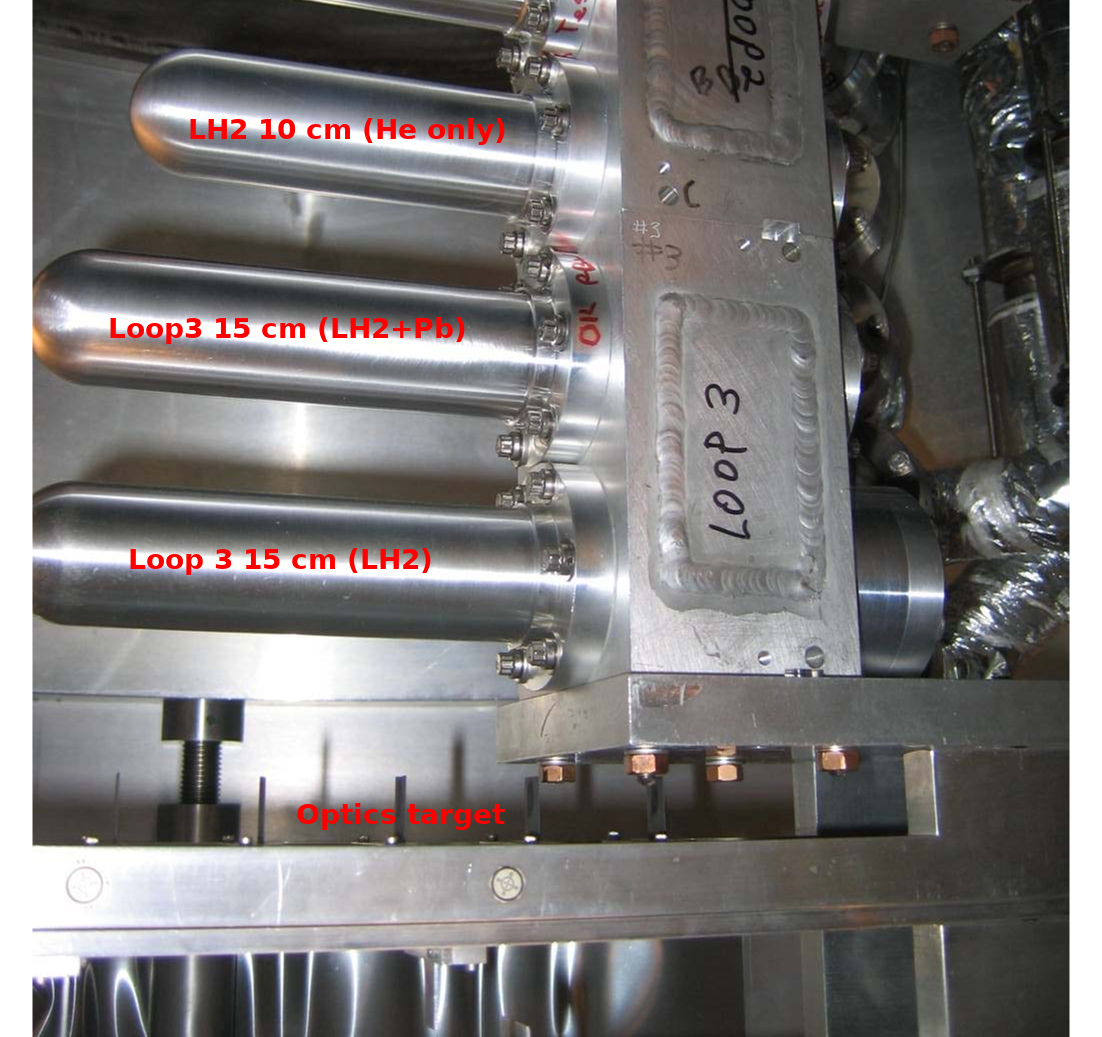
\includegraphics[width=0.8\textwidth]{figs/Loop2_Loop3_target_edit.png}
\caption[Loop 2 and Loop 3 cryogenic target ]{Loop 2 and Loop 3 cryogenic target. }\label{fig:loop2_loop3}
\end{figure}

%solid target

Next in the ladder are optics, dummy and empty targets (see Figure.\ref{fig:optics_dummy}).
The optics target are 7 carbon foils cut from the same 99.5\% chemically pure carbon sheet.
The thickness of each foil is 0.042 $\pm$ 0.001 g/cm$^2$, they are separated by 4 cm along the beam $\hat{z}$ direction.

\begin{figure}[tb!]
\centering
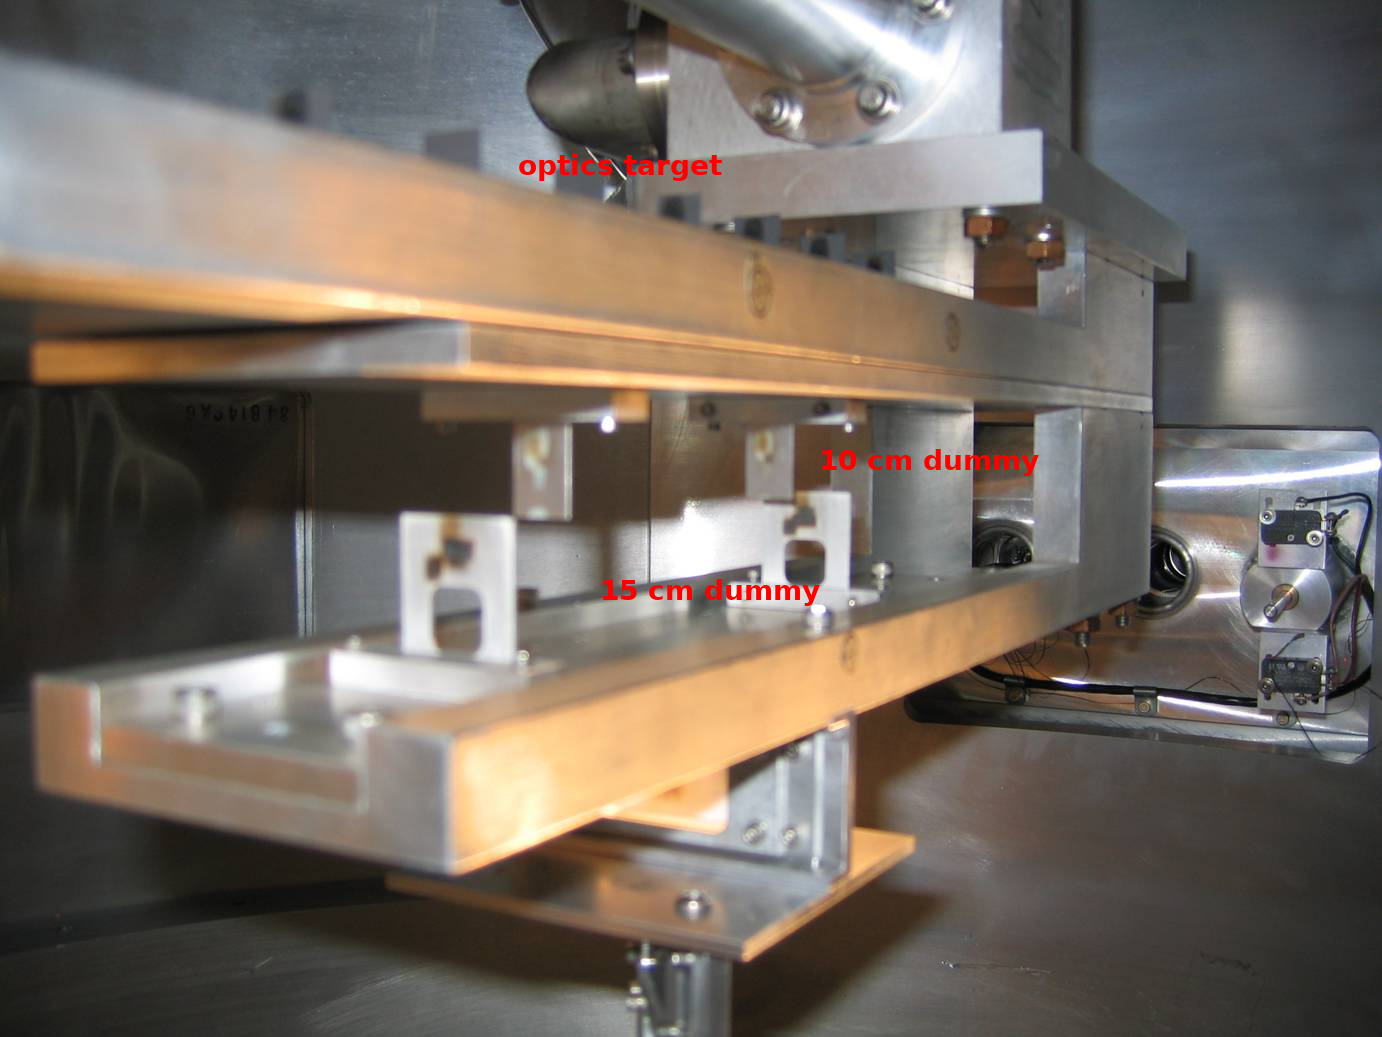
\includegraphics[width=0.8\textwidth]{figs/optics_dummy_target_edit.png}
\caption[Optics, dummy and empty target ]{Optics, dummy and empty target. }\label{fig:optics_dummy}
\end{figure}

The dummy targets are two pairs of aluminum foils with thickness 0.259 $\pm$ 0.001 g/cm$^2$.
One pair are separated by 10 cm in $\hat{z}$ direction (called "10 cm dummy target"), and another pair are separated by
15 cm in $\hat{z}$ direction (called "15 cm dummy target"), to measure the contribution from the window
of cryogenic targets.  There is a hole on each foil of the second dummy target, which is called "empty target".

The last on the target ladder are solid targets.
The upper position is for BeO which is perpendicular to the beam.
The second two positions are for carbon and iron targets and they are tilted \SI{51.78}{\degree}
clockwise when viewed from top, so the beam hits the right side of foils.
The bottom two positions are also for carbon and iron targets, but tilted \SI{48.56}{\degree}
counterclockwise, and the beam hit the foils from the left side. The configuration of the left and right titled solid
target are shown in Figure ~\ref{fig:left_right_tilted_target}.
%This design makes the electrons travel different length in target after scattering before
%they enter one or the other spectrometer. Therefore, by comparing the spectra from both HRSs,
%we can study the external radiative effect.
The solid targets are shown in Figure.\ref{fig:carbon_iron}.

\begin{figure}[tb!]
\centering
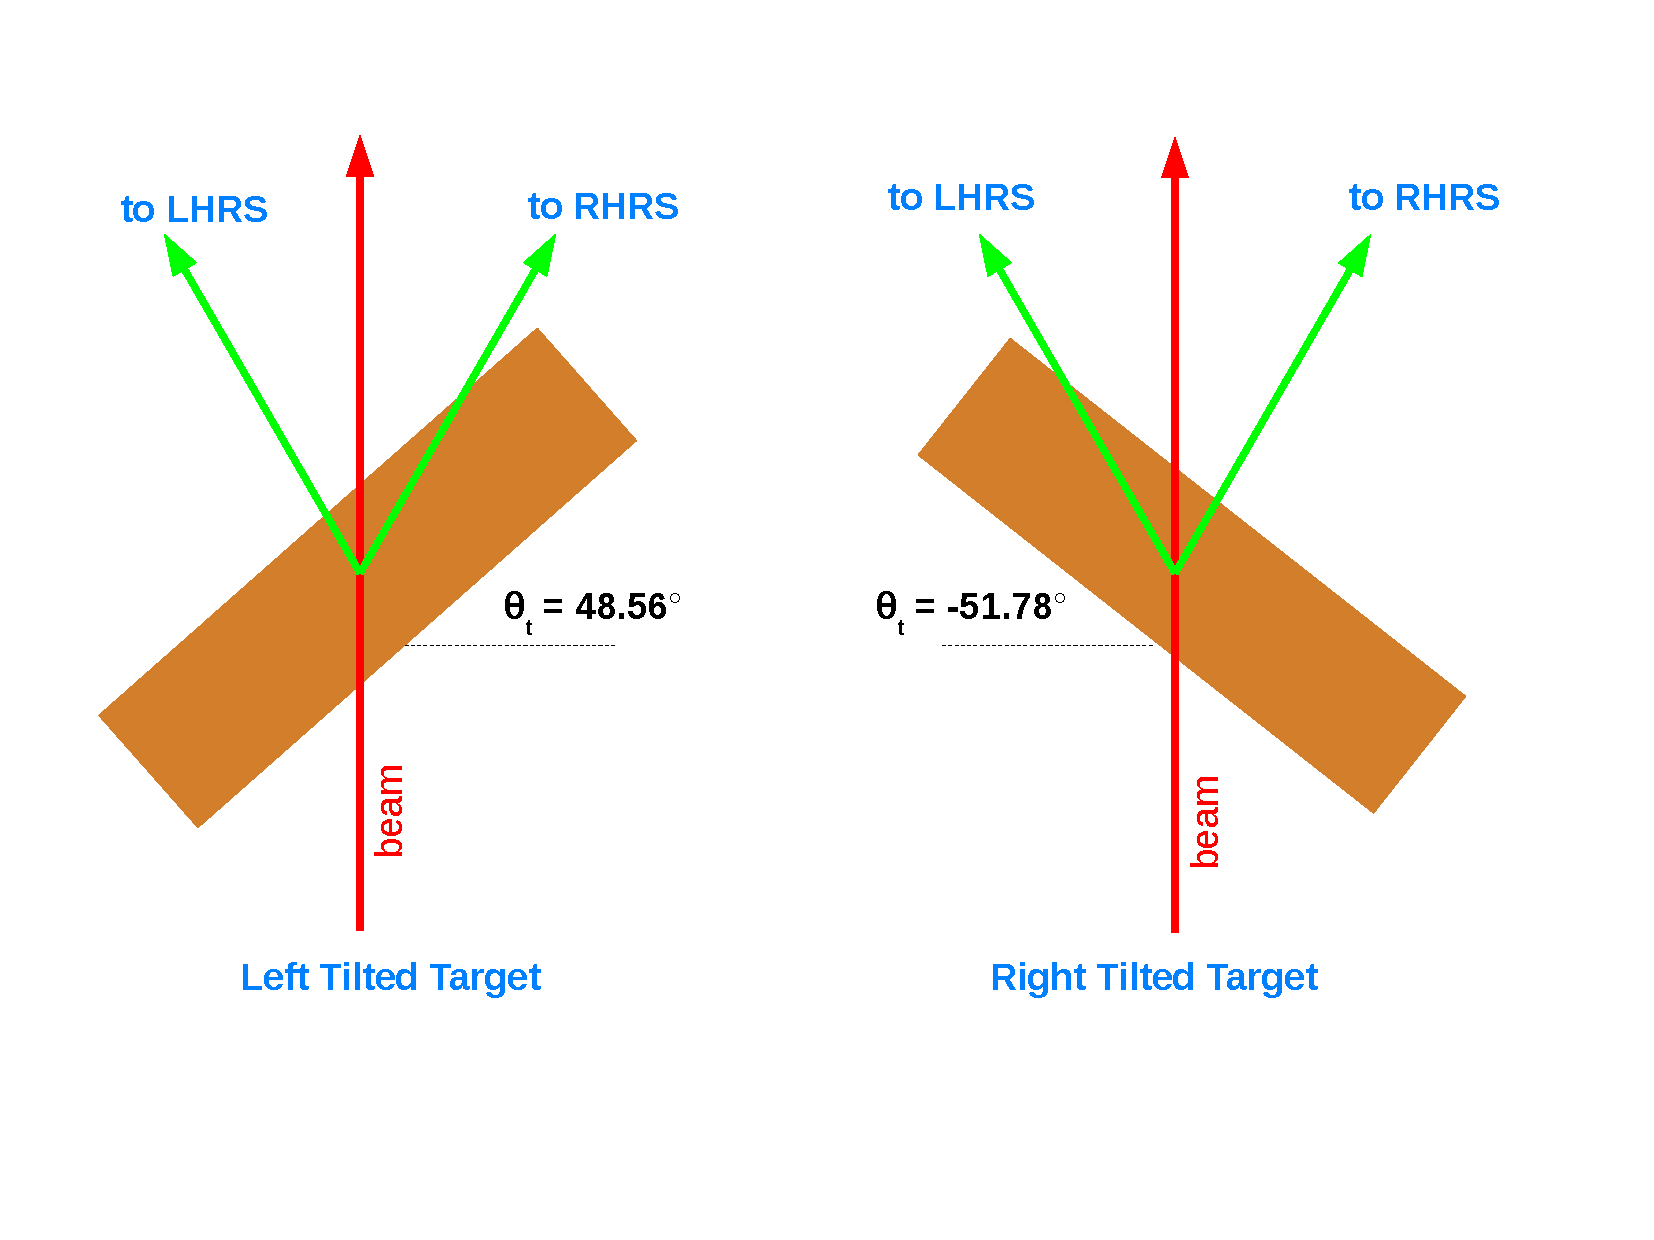
\includegraphics[width=0.8\textwidth]{figs/left_right_tilted_target.pdf}
\caption[left right tilted target ]{Configuration of left and right tilted target(viewed from the top). }\label{fig:left_right_tilted_target}
\end{figure}

\begin{figure}[tb!]
\centering
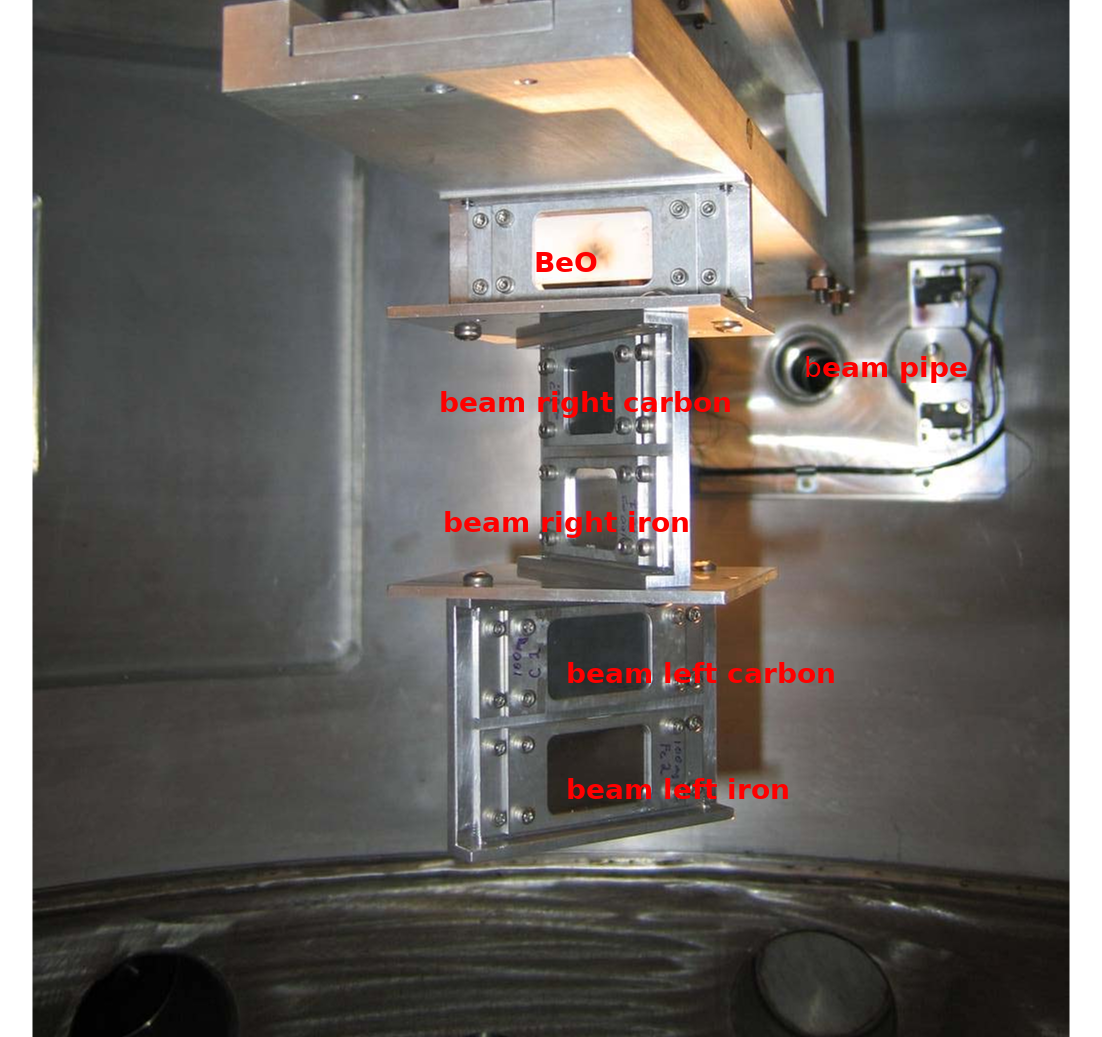
\includegraphics[width=0.8\textwidth]{figs/carbon_iron_target_edit.png}
\caption[Solid targets ]{Solid targets. }\label{fig:carbon_iron}
\end{figure}

Table.\ref{tab:purity_thickness} gives the target foil positions, thicknesses and chemical purities.

\begin{table}[tb!]
\centering
\begin{tabular}{|l|r|r|r|}
\hline
Purity  & Target Position   & Material & Thickness ($g/cm^2$) \\ \hline
99\%    & BeO               & BeO      & 0.149 $\pm$ 0.001    \\ \hline
99.95\% & Beam right carbon & Carbon   & 0.0894 $\pm$ 0.0001  \\ \hline
99.99\% & Beam right iron   & Iron     & 0.1027 $\pm$ 0.0001  \\ \hline
99.95\% & Beam left carbon  & Carbon   & 0.0895 $\pm$ 0.0001  \\ \hline
99.99\% & Beam left iron    & Iron     & 0.1023 $\pm$ 0.0001  \\ \hline
\end{tabular}
\caption[Solid target purity and thickness]{Solid target purity and thickness}\label{tab:purity_thickness}
\end{table}


\section{Hall A High-Resolution Spectrometers}
The core of the Hall A equipment is a pair of nearly identical spectrometers that can reach a maximum momentum bend of
4 GeV/$c$. These spectrometers were
designed to study electromagnetic interactions and hadronic structure with high precision.
Their basic layout is shown in Fig~\ref{fig:HRS_spectrometer}.
Important design characteristics of spectrometer are shown in the Table~\ref{tab:HRS_chars}.



\begin{figure}[tb!]
\centering
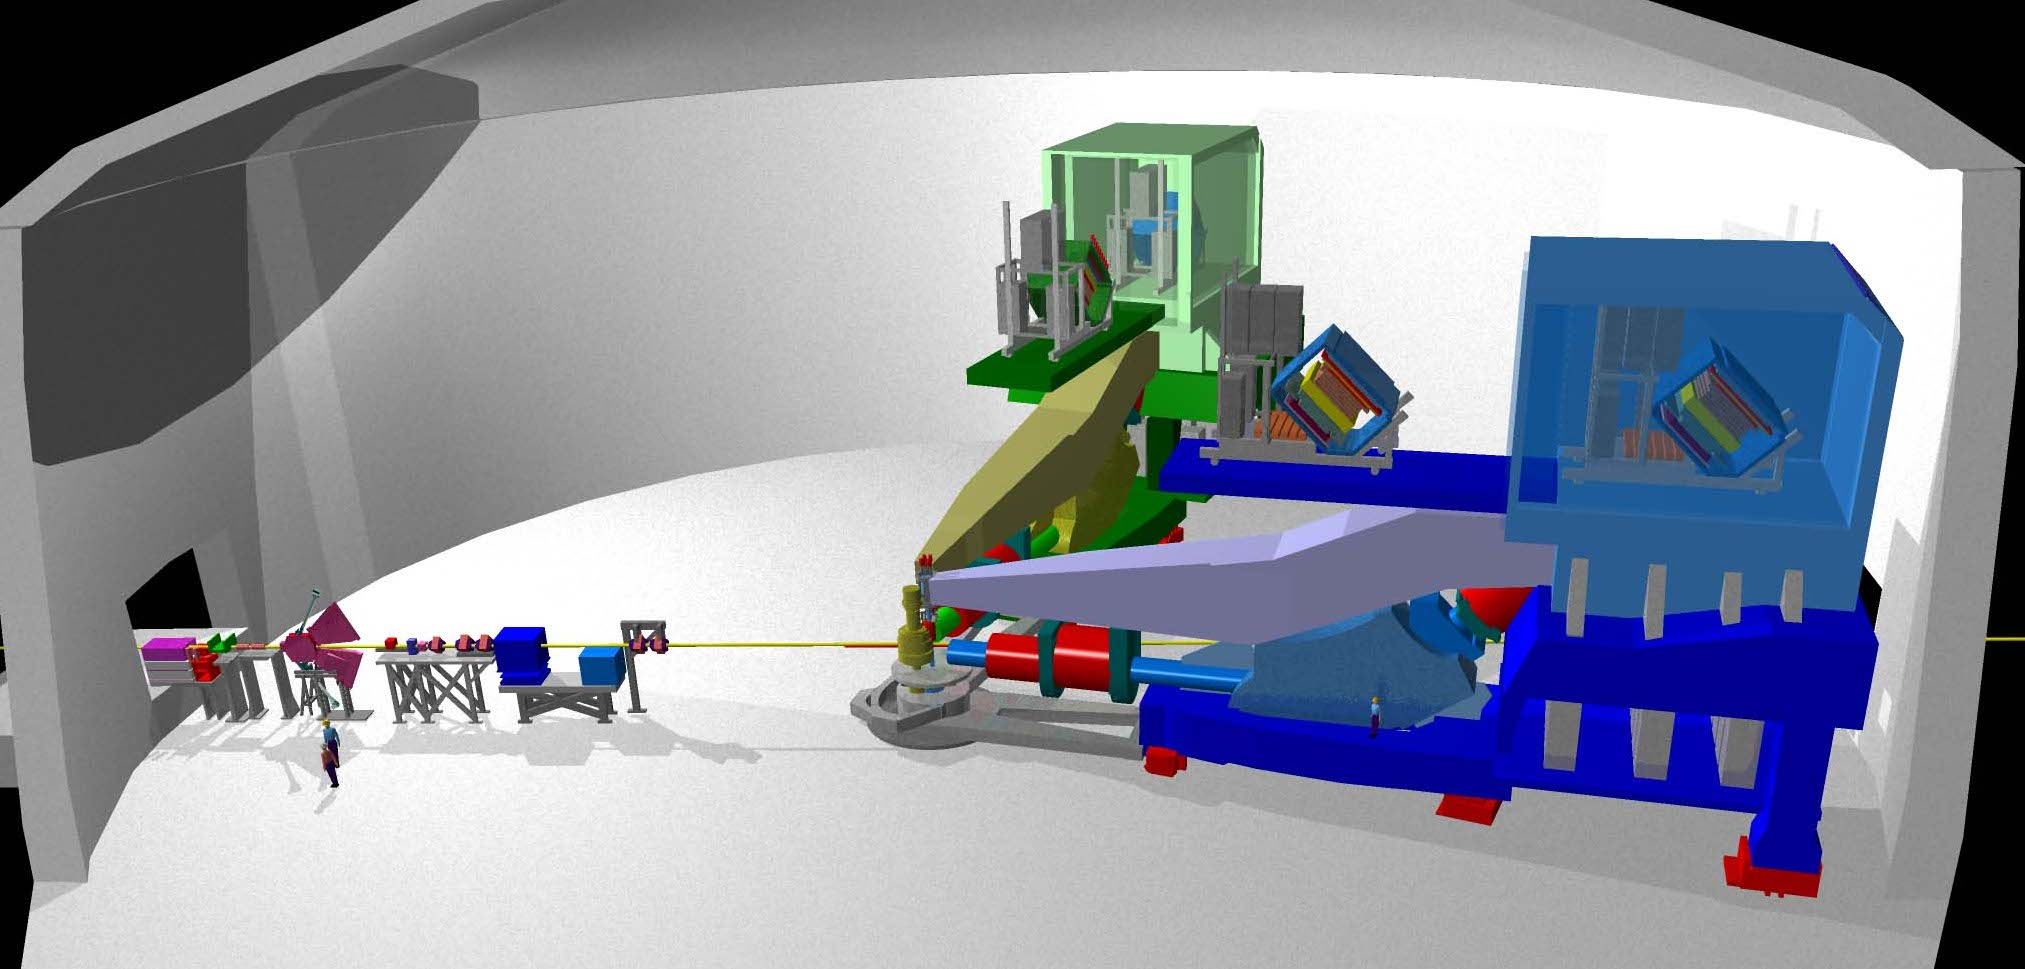
\includegraphics[width=0.9\textwidth]{figs/HRS_spectrometer.png}
\caption[Hall A HRS spectrometer]{The Hall A high resolution spectrometers.  \label{fig:HRS_spectrometer}}
\end{figure}

\begin{table}[tb!]
\begin{tabular}{ll}
\hline
Configuration                         & QQDQ vertical bend                  \\
Bending angle                         & \SI{45}{\degree}                    \\
Optical length                        & 23.4 m                              \\
Momentum range                        & 0.1 - 4.0 GeV/$c$                   \\
Momentum acceptance                   & -4.5 \% $<$ $\delta$p/p $<$ +4.5 \% \\
Momentum resolution                   & 1 $\times$ 10$^{-4}$                \\
Dispersion at the focus (D)           & 12.4 m                              \\
Radial linear magnification (M)       & -2.5                                \\
D/M                                   & 5.0                                 \\
Angular range                         &                                     \\
HRS-L                                 & 12.5 - \SI{150}{\degree}            \\
HRS-R                                 & 12.5 - \SI{130}{\degree}            \\
Angular acceptance                    &                                     \\
Horizontal ($\phi$)                   & $\pm$ 30 mrad                       \\
Vertical ($\theta$)                   & $\pm$ 60 mrad                       \\
Angular resolution                    &                                     \\
Horizontal ($\Delta\phi/\phi$)        & 0.5 mrad                            \\
Vertical ($\Delta\theta/\theta$)      & 1.0 mrad                            \\
Solid angle at $\delta$p/p=0, $y_0$=0 & 6 msr                               \\
Transverse length acceptance          & $\pm$ 5 cm                          \\
Transverse position resolution        & 1 mm                                \\ \hline
\end{tabular}
\caption[Main design characteristics of the Hall A high resolution spectrometers]
{Main design characteristics of the Hall A high resolution spectrometers.}\label{tab:HRS_chars}
Table reproduced from \cite{Alcorn2004}.
\end{table}


\subsection{Design and Characteristics of the Magnets}
Each HRS spectrometer has four superconducting magnets: three quadruples and one dipole.
The QQDQ magnet configuration (see Figure~\ref{fig:QQDQ_config}) (Q stands for quadruple and D stands for dipole) is used for a few requirements:
a high momentum resolution at the 10$^{-4}$ level over the 0.8 to 4.0 GeV/$c$ momentum range, a large acceptance
in both angle and momentum, good position and angular resolution in the scattering plane, and extended target
acceptance \cite{Alcorn2004}.
The first two quadruples are used to focus the scattered electrons vertically and horizontally, respectively,
to achieve the desired angular acceptance and avoid particles to collide with the magnets.
The dipole is mainly used to bend the electron trajectory \SI{45}{\degree} upward and to achieve a good
momentum resolution. The third quadruple will further focus beam horizontally. 

\begin{figure}[tb!]
\centering
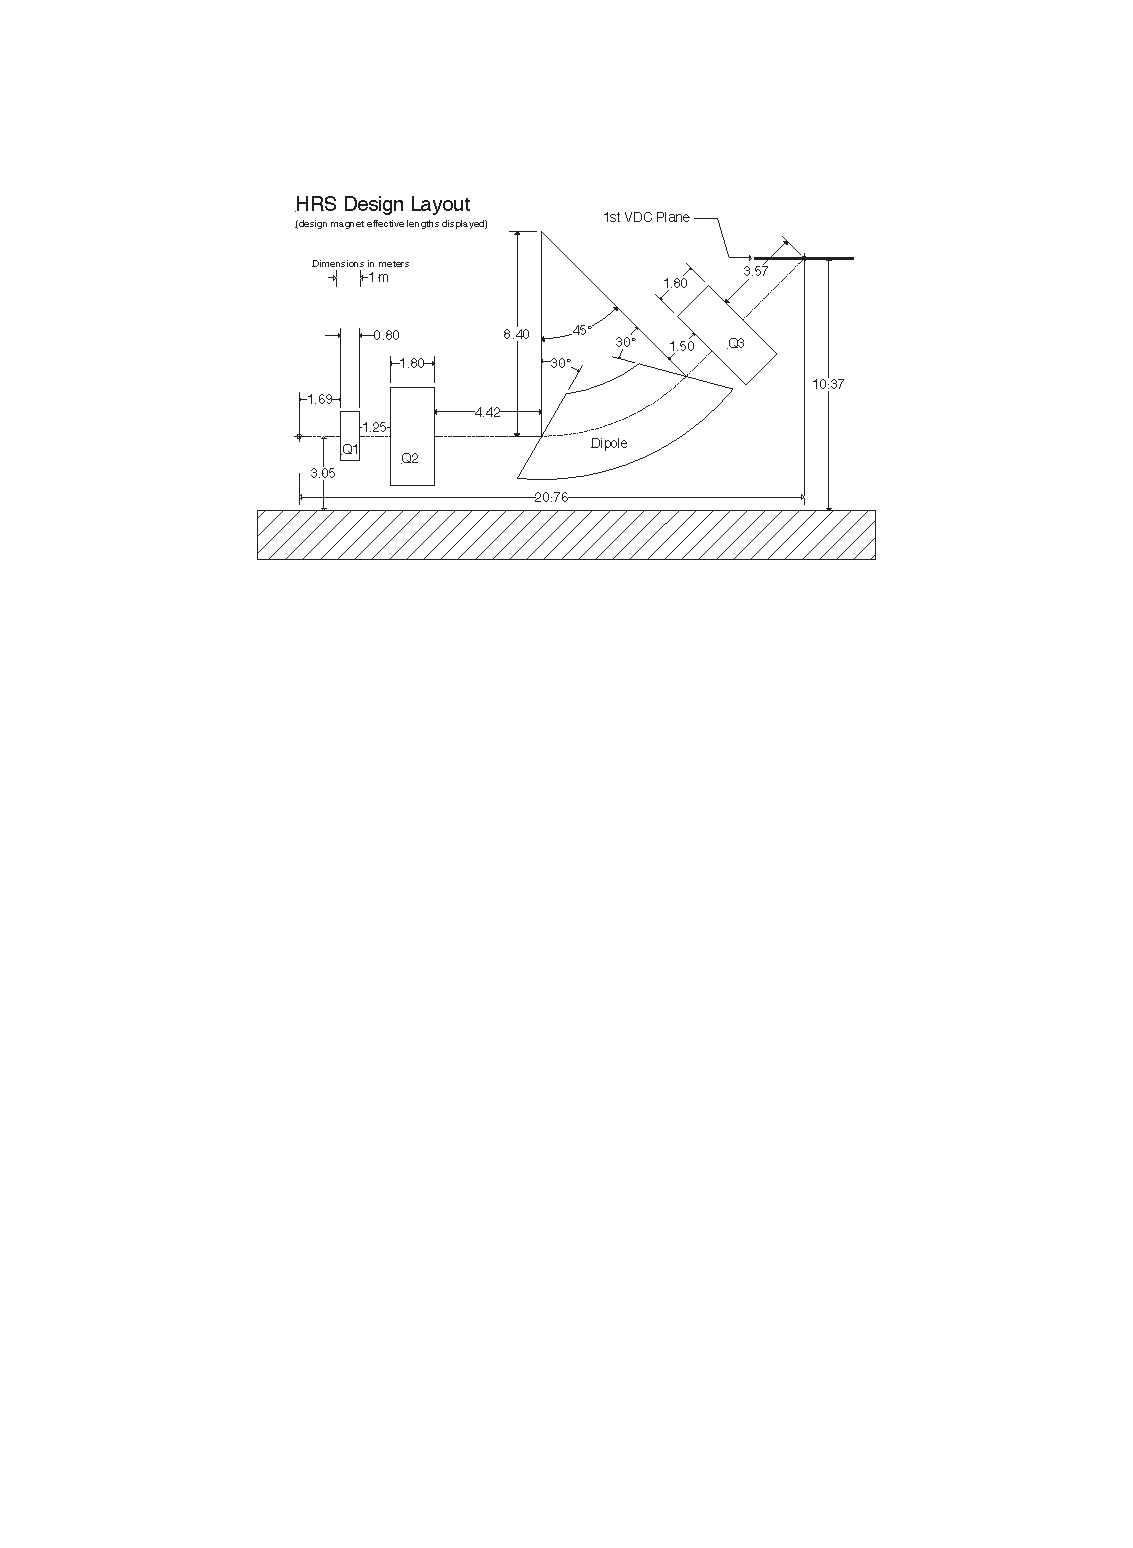
\includegraphics[width=0.9\textwidth]{figs/HRS.pdf}
\caption[HRS magnets layout]{The Hall A high resolution spectrometers magnets layout(sideview).  \label{fig:QQDQ_config}}
\end{figure}

\subsection{Collimator}
Each HRS spectrometer has a collimator box carefully aligned and rigidly attached to the entrance flange of the 
first quadruple.
In each collimator box, there are a set of collimators and a sieve slit.

The first two collimators are made of 80 mm thick tungsten, positioned around 1109 mm away from the target.
The first collimator has an aperture of 121.8(vertical) $\times$ 62.9(horizontal) mm at the entrance and
129.7(V) $\times$ 66.8(H) mm at the exit.
The second collimator is smaller and with an aperture of 50.0(V) $\times$ 21.3(H) mm at the entrance and 53.2(V) $\times$
22.6(H) mm at the exit.

The third collimator is called "sieve slit", which is used to determine the angular information during optics calibration.
It is made of 5 mm thick stainless steel sheet, positioned 1165.3 mm (LHRS) (or 1192.5 mm (RHRS)) away from Hall A center.
There are 49 holes (arranged in a 7$\times$7 array) on the sieve slit, spaced 25 mm apart vertically and 12.5 mm part horizontally.
Two of them big holes, one in the center and one displaced two rows vertically and one horizontally, are 4 mm in
diameter. The other holes are 2 mm in diameter.

\subsection{Detector Packages}
Following the third quadruple is the detector package.
The detector package is designed for various functions in the characterization of charged particles coming through the spectrometer.
For CSR experiment the detector package includes:

\begin{itemize}
\item A pair of Vertical Drift Chambers (VDCs) to determine the tracking information (momentum and trajectory);
\item Two scintillator planes, S1 and S2, to provide trigger to activate the data acquisition(DAQ) electronics;
\item A gas Cerenkov detector to provide particle identification (PID) information;
\item On LHRS, there is a NaI calorimeter to extract information on low energy electrons. 
Unfortunately, some blocks are unresponsive during the experiment due to the unsuccessful installation.
So the NaI was not used for data analysis.
\item A set of lead glass calorimeter for additional PID.
\end{itemize}

The layout of the LHRS and RHRS detector packages are shown in Figure.~\ref{fig:LHRS_detectors} and
Figure.~\ref{fig:RHRS_detectors}. The details of the detectors used in CSR experiment are explained below.

\begin{figure}[tb!]
\centering
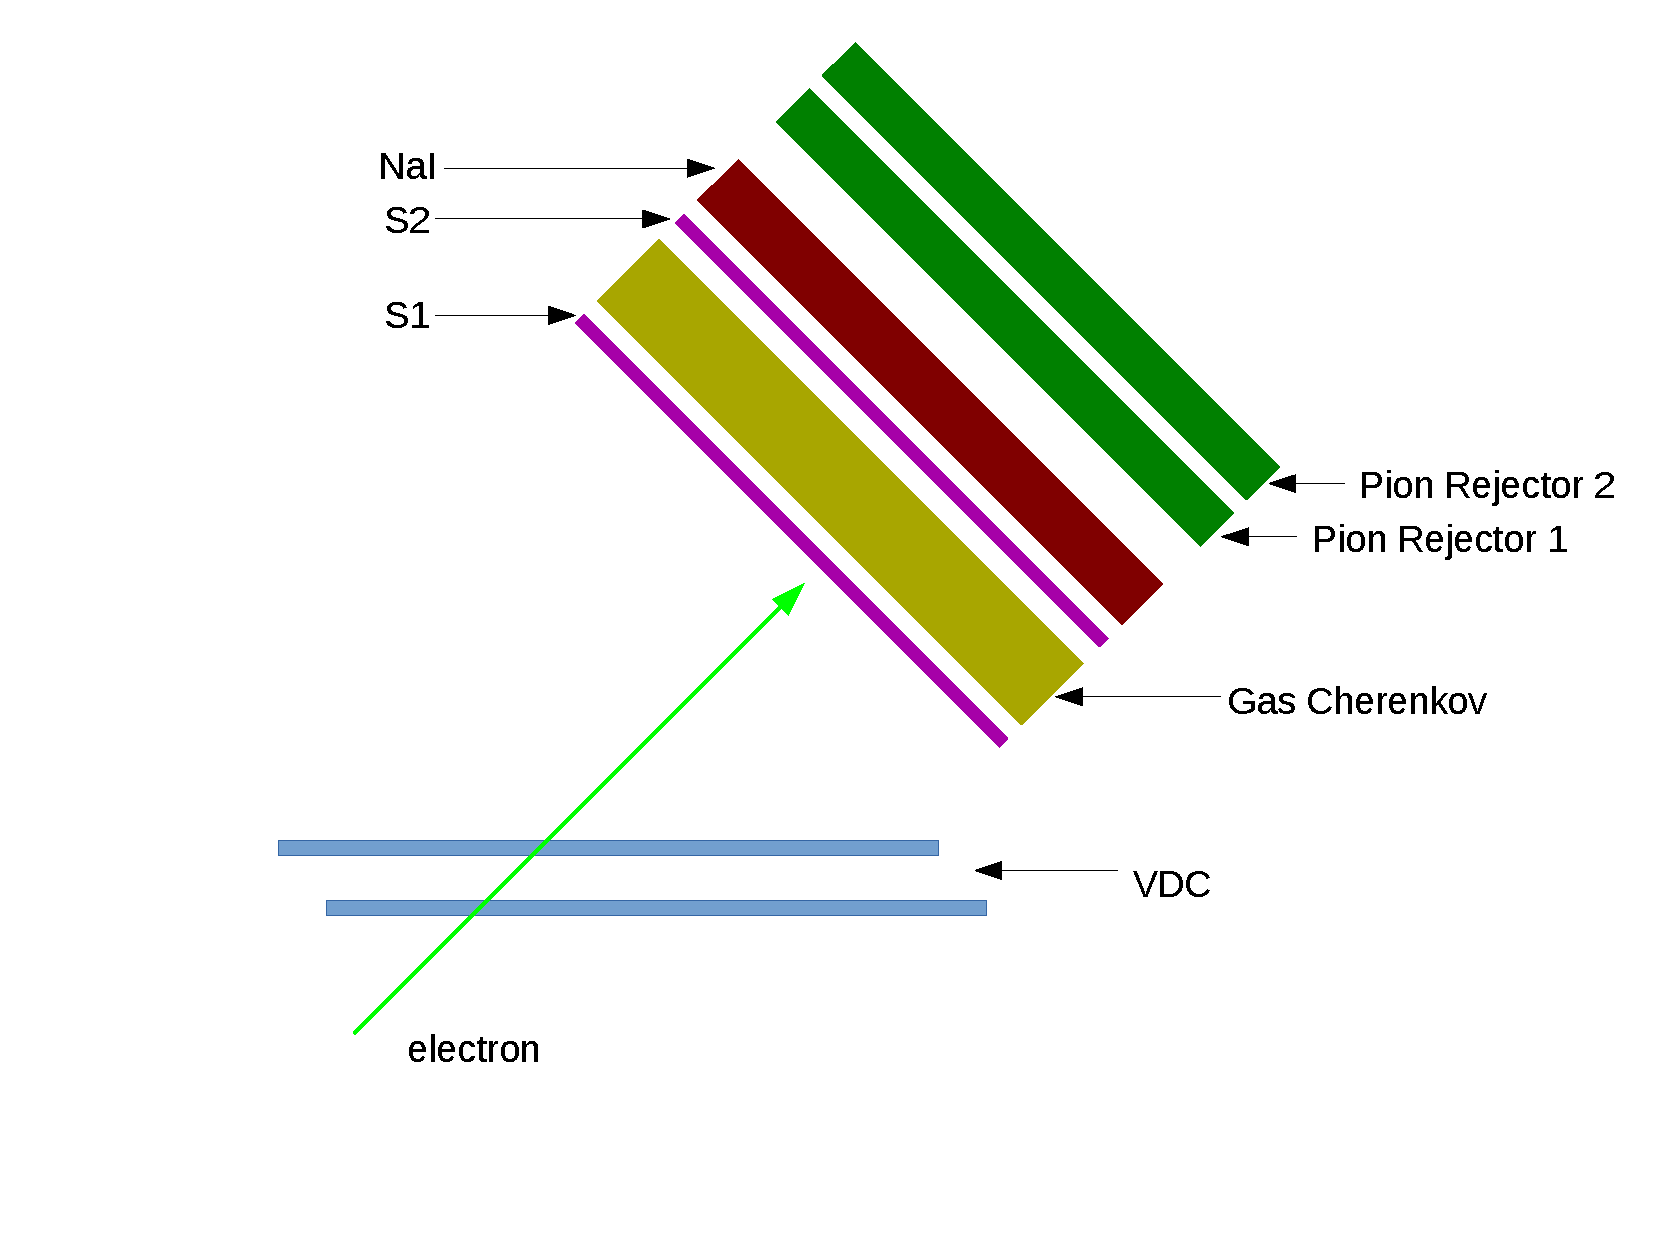
\includegraphics[width=0.5\textwidth]{figs/LHRS_detectors.pdf}
\caption[The LHRS detector package.]{The LHRS detector package.  \label{fig:LHRS_detectors}}
\end{figure}

\begin{figure}[tb!]
\centering
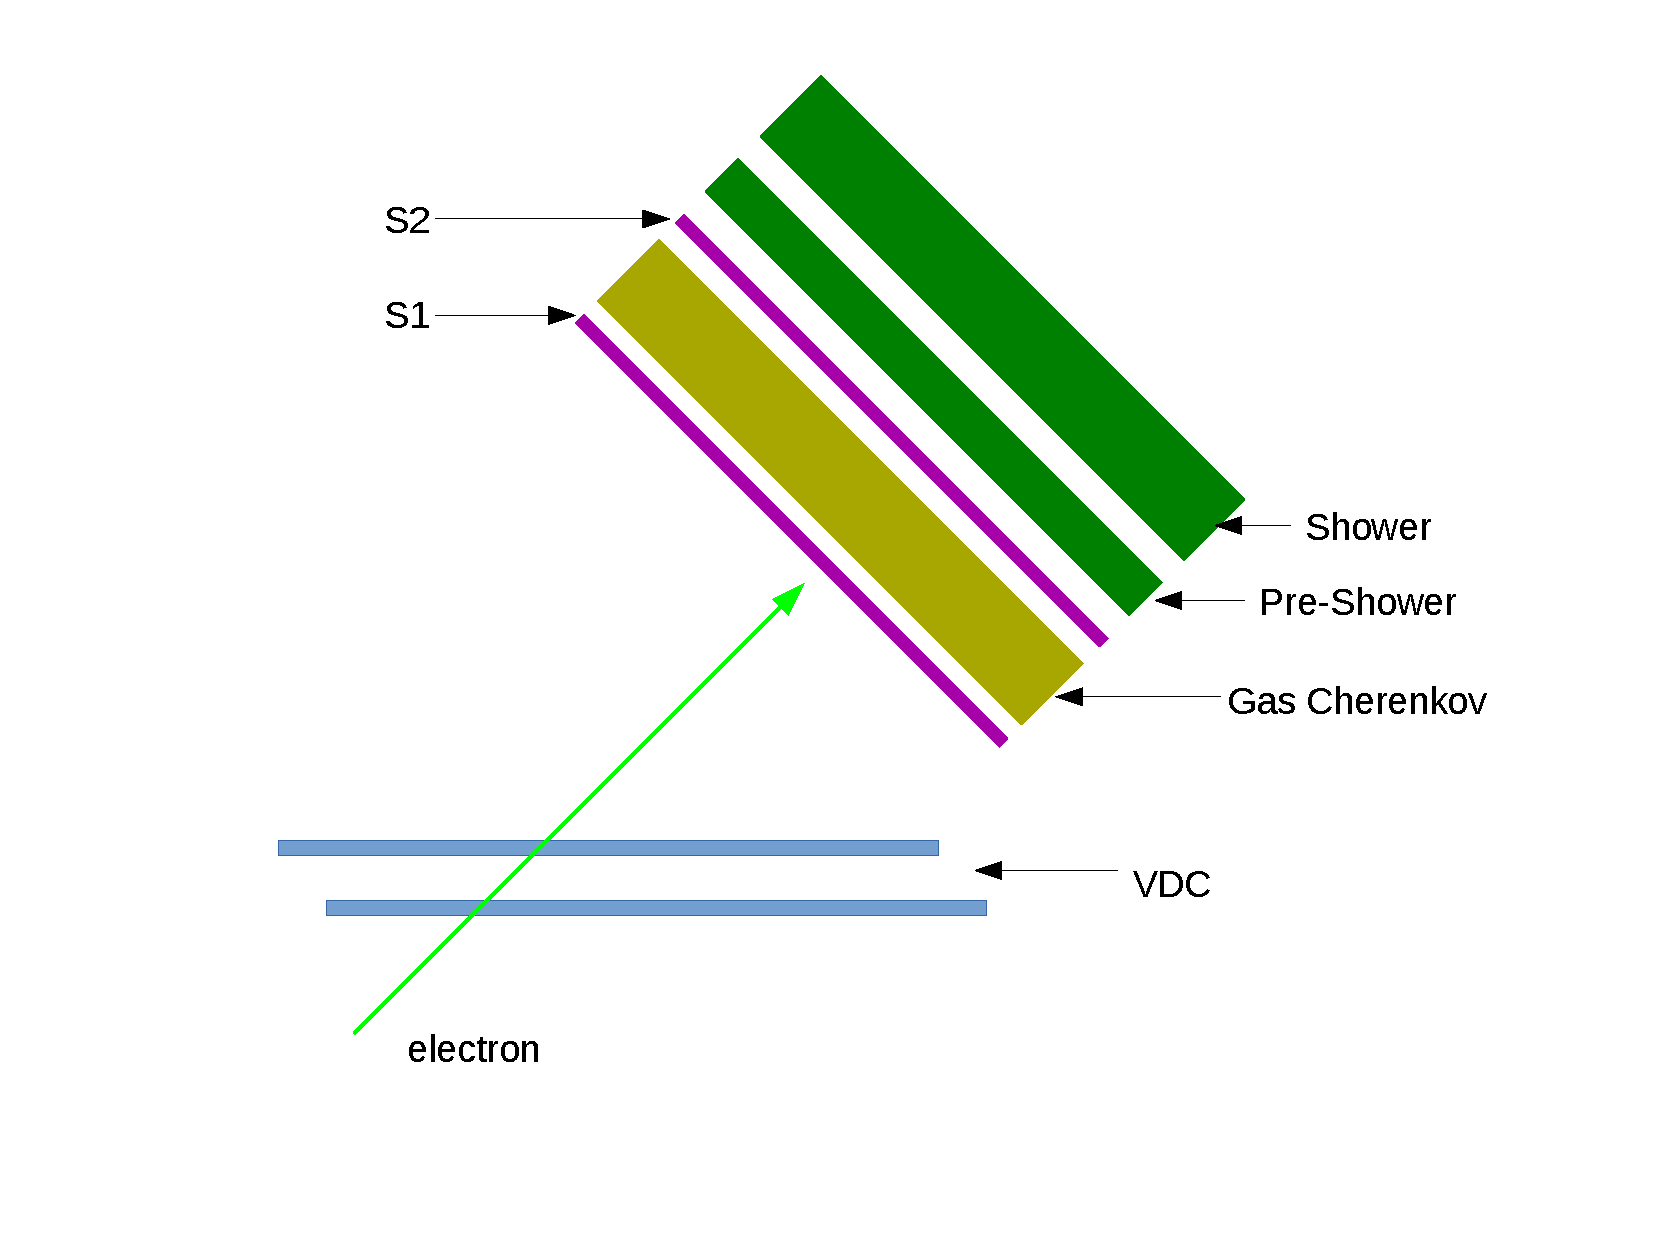
\includegraphics[width=0.5\textwidth]{figs/RHRS_detectors.pdf}
\caption[The RHRS detector package.]{The RHRS detector package.  \label{fig:RHRS_detectors}}
\end{figure}


\subsubsection{Vertical Drift Chamber}
%position and geometry
Each HRS spectrometer use a pair of Vertical Drift Chambers (VDC) to provide particle tracking information.
The layout of VDC is shown in Figure.~\ref{fig:VDC_layout}.

\begin{figure}[tb!]
\centering
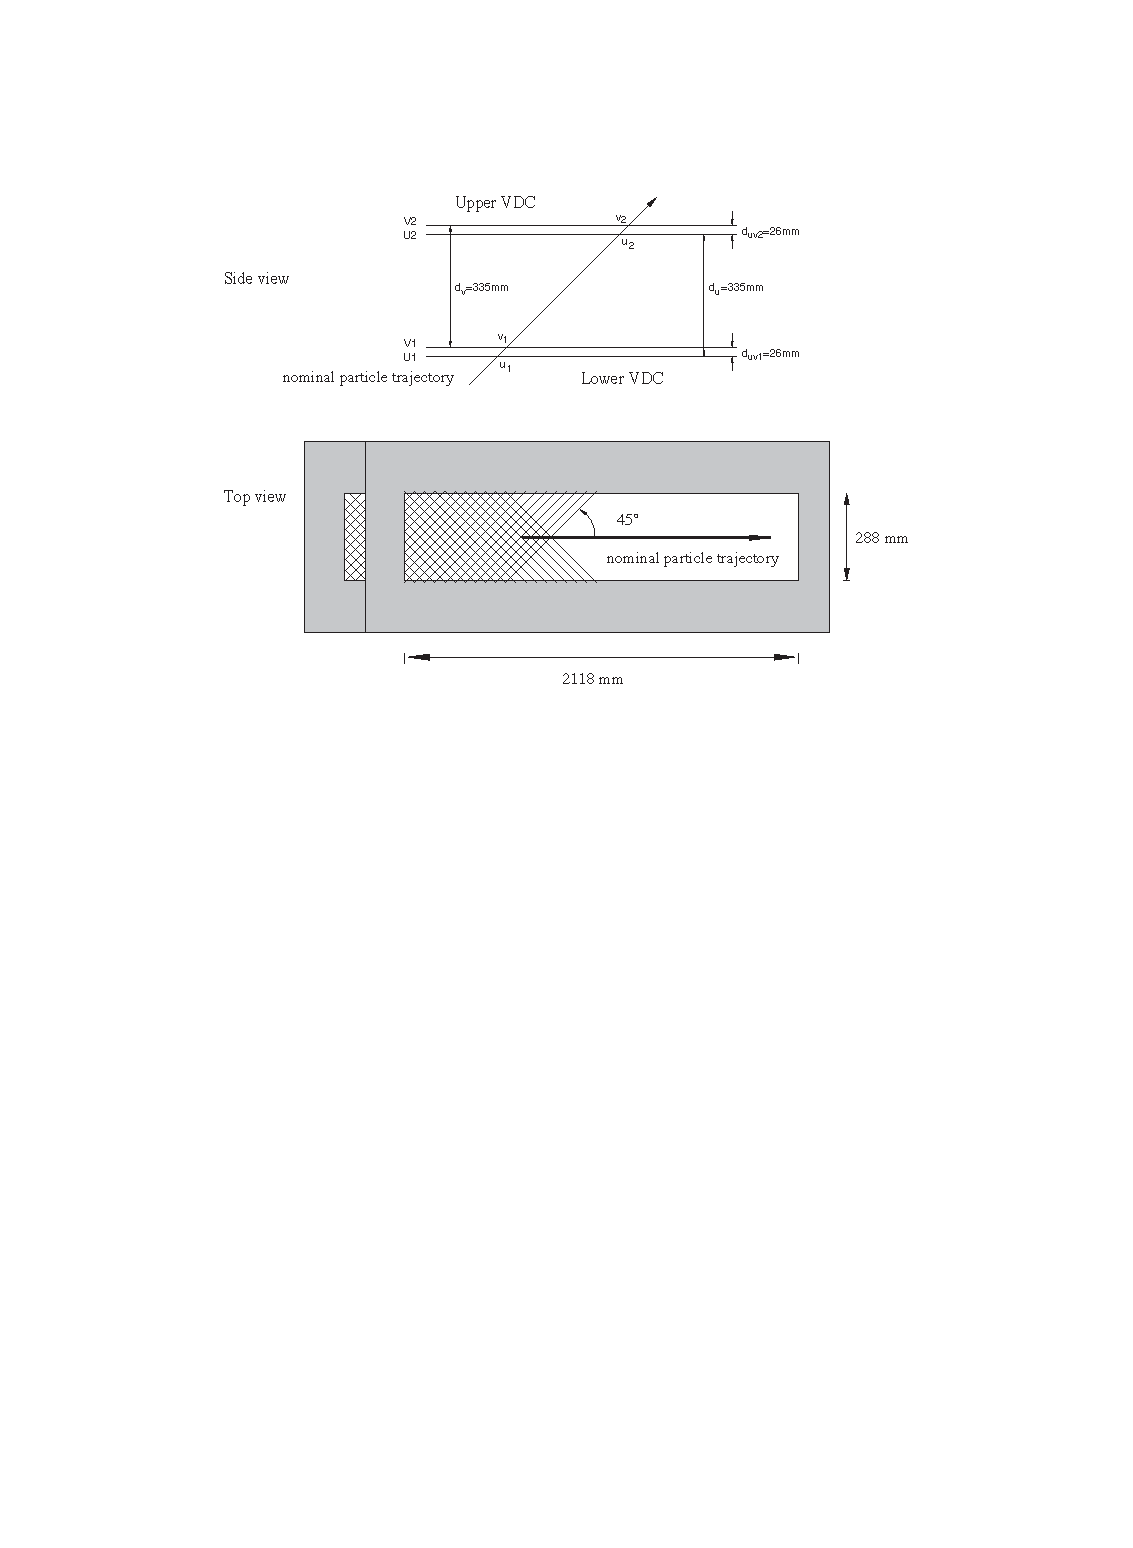
\includegraphics[width=0.8\textwidth]{figs/VDC.pdf}
\caption[Schematic layout of Vertical Drift Chambers]{Schematic layout of a pair of Vertical Drift Chambers.
\label{fig:VDC_layout}}
\end{figure}

The two VDC chambers are positioned 335 mm away from each other, each VDC has a standard U-V plane configuration.
The wires of one plane are \SI{90}{\degree} to that of the other plane, and lie in the laboratory horizontal plane.
They are inclined at an angle of \SI{45}{\degree} with respect to the dispersive(vertical) and non-dispersive(horizontal) directions.
The particle's central trajectory crosses the wire planes at an angle of \SI{45}{\degree}.
The distance between U and V planes is 26 mm, there are 368 sense wires in each plane, the spacing between two
adjacent wire is 4.243 mm.

%volt, gas, and signal
There are three high voltage gold-plated Mylar planes at about -4 kV in each VDC, one between U and V wire planes and two on opposite
sides, the wires are kept at ground voltage. The electric field between wires and cathode plane is show in Figure~\ref{fig:wire_chamber}.
The gas supply to the VDCs is a 62\% argon and 38\% ethane mixture. The gas is bubbled through cooled alcohol to reduce
aging effects on the sense wires \cite{Alcorn2004}. 

\begin{figure}[tb!]
\centering
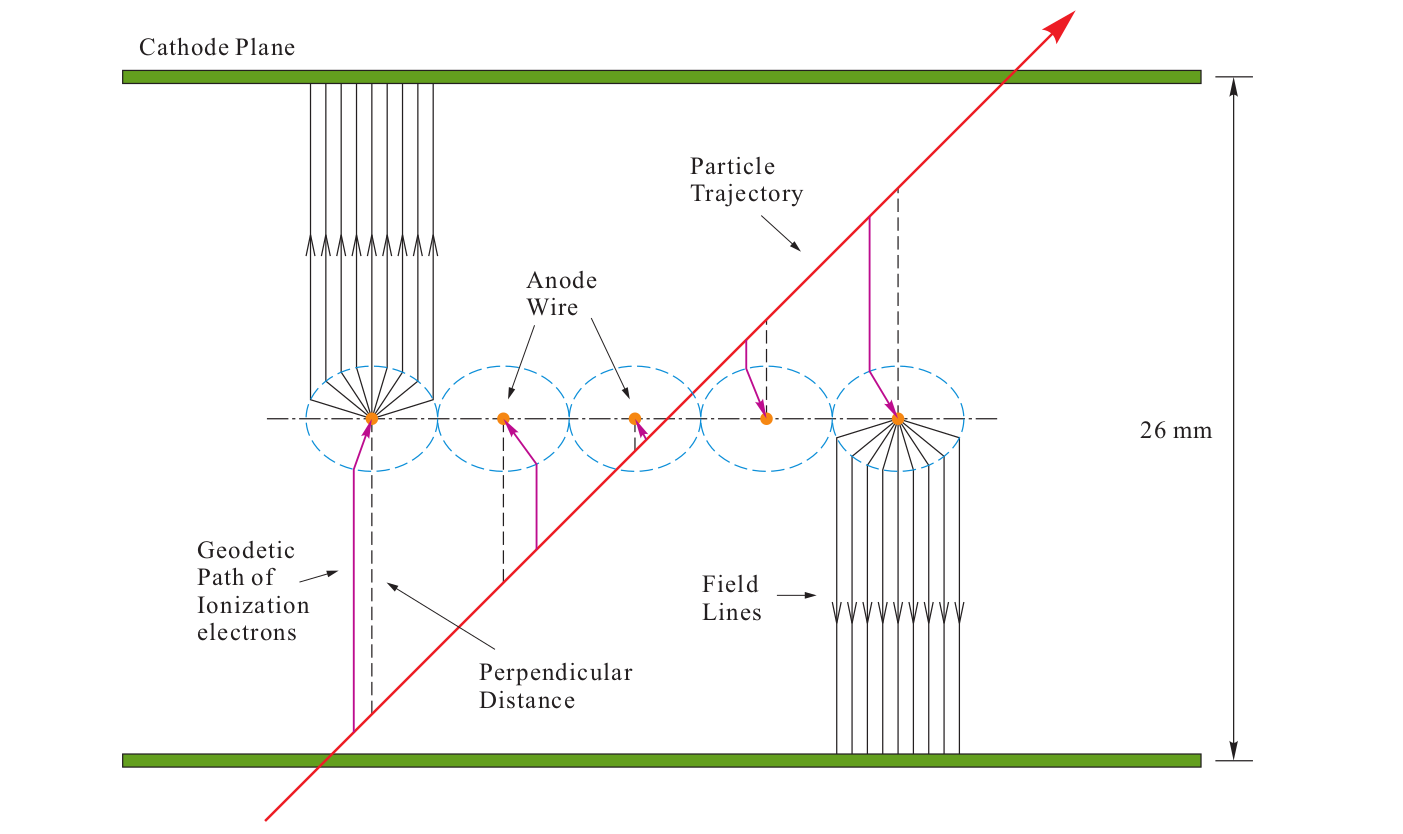
\includegraphics[width=0.8\textwidth]{figs/wire_chamber.png}
\caption[wire chamber]{Electric field between wires and cathode plane in VDC.
\label{fig:wire_chamber}}
\end{figure}

When an electron passes through the VDC planes, it ionizes the gas inside the chamber and leave behind ions and
generated electrons on it track. The generated electrons are drifted towards the sense wires with a constant velocity
(50 $\mu$m/ns) along the path of the least time, and accelerate rapidly near the wire producing a shower of secondary ionization.
This generates an electric signal on the sense wires. The timing information of the signal is measured by the Time-To-Digital
Converter (TDC), which is started by a triggered wire and stopped by the event trigger supervisor.
Since the ionization electron drift velocity is constant, the drift distance from trajectory to the wire can be
extracted from the TDC output. The trajectory can be reconstructed by combining drift distances of all fired wires.
By design, the charged particle crosses the VDCs at the nominal angle of \SI{45}{\degree} typically triggers 5 wires.
Considering the inefficiency of sense wires, the signals from 3 hits are also accepted as good track. 
The position and angular reconstruct resolution of focal plane are approximately 100 $\mu$m and 0.5 mrad, respectively.

\subsubsection{Scintillators and Trigger}
Two scintillator planes, S1 and S2, separated by 2 m, are used to generate the trigger for the DAQ system.
The active volume dimension of S1 and S2 are 36.0 cm (transverse or horizontal direction) $\times$ 29.3 cm (dispersive
or vertical direction) $\times$ 0.5 cm (thickness), and 60.0 cm (horizontal) $\times$ 37.0 cm (vertical) $\times$ 0.5
cm (thickness), respectively.
Each scintillator consists of 6 overlapping scintillator paddles made of thin plastic scintillators. 
Two photomultipliers (PMT) are attached to each scintillator paddle, one on left side and another on right side.
The time resolution of each plane is around 0.3 ns.

Charged particles coming through a scintillator paddle may generate scintillating light which travels towards
PMTs on both sides. Signals from PMTs are used to generate triggers and sent to all other detectors and the DAQ system.
To select good events for the analysis, each event is assigned an event type, with values from 1 to 5, based on the 
the scintillator signals as follows: 

\begin{itemize}
\item A T1(T3) event for the right(left) arm is considered to be a "good event". It satisfies the following conditions:
  \begin{enumerate}
    \item A scintillator paddle is called "fired" if PMTs on its both sides have signals;
    \item The N$_1$$^{th}$ paddle of S1 and N$_2$$^{th}$ paddle of S2 are "fired" within a specific time window;
    \item N$_2$$^{th}$ = N$_1$$^{th}$ or N$_2$$^{th}$ = N$_1$$^{th}$ $\pm$ 1. This means the angle formed by the particle trajectory
    and the central ray of the spectrometer is very small, or the trajectory is at approximately \SI{45}{\degree} with respect to the Hall floor.
  \end{enumerate}

 \item A T2(T4) event for the right(left) arm is formed if \textit{one of} the follwing conditions is satisfied:
  \begin{enumerate}
  \item The N$_1$$^{th}$ of S1 and N$_2$$^{th}$ of S2 are fired at the same time, but
        N$_2$$^{th}$ $\neq$ N$_1$$^{th}$ and N$_2$$^{th}$ $\neq$ N$_1$$^{th}$ $\pm$ 1;
  \item Either S1 or S2 is fired, at the same time Gas Cerenkov fires.
  \end{enumerate}
  T2(T4) events are either cosmic ray events, or particles on the edge of the acceptance.

 \item A T5 event is defined as the coincidence event of T1 and T3. It was not used during the CSR experiment.
\end{itemize}

Triggers T1-T4 are counted by scalers and are sent to the trigger supervisor. The trigger supervisor sychronizes all the
detector read-out and send them to the DAQ system. Because of the hardware limitation of DAQ system, it cannot record all
events when event rate is high. A quantity called livetime(LT) is defined as the fraction of events
recorded by DAQ, given by:

\begin{equation} \label{LT_def}
LT = \frac{\mathrm{number \; of \; events \; that \; are \; recorded \; by \; DAQ}}{\mathrm{number \; of \; events \; that \; are \; fed
\; to \; DAQ}}
\end{equation}
If the event rate is very high, events can be prescaled by an integer prescale factor $p_{1(2,3,4)}$ for $T_{1,2,3,4}$ at the trigger supervisor to decrease the
load of DAQ system. Only one event is sent to the DAQ system for each set of $p_{1(2,3,4)}$ subsequent events.
Livetime is event type dependent. It can be found by comparing the number of triggers $T_{1(2,3,4)}$ recorded by scalers
and the total number of triggers accepted by the DAQ system, $T_{DAQ,1(2,3,4)}$:

\begin{equation}
LT_{1,(2,3,4)} = \frac{p_{1,(2,3,4)}T_{DAQ,1(2,3,4)}}{T_{1(2,3,4)}}
\end{equation}  

Similarly, we can define a quantity called trigger inefficiency which describes the fraction of 
"good events" miscounted as T2(T4) events.
To minimize the dilutions from cosmic events, we usually choose a high yield run.
The trigger inefficiency is defined as:

\begin{equation}
\mathrm{Inefficiency} = \frac{T_{2(4)}}{T_{1(3)} + T_{2(4)}}
\end{equation}  

Then the trigger efficiency can be extracted as:

\begin{equation}
\eta_{trig} = 1 - \mathrm{Inefficiency} =  \frac{T_{1(3)}}{T_{1(3)} + T_{2(4)}}
\end{equation}  

The trigger inefficiencies for both left and right arms are below 1\% during CSR experiment
and are negligible.


\subsubsection{Gas Cerenkov Detector}
Gas Cerenkov detector is used for particle identification in CSR experiment.
The Gas Cerenkov detector is based on Cerenkov effect.
When a charged particle passing through a dielectric medium with a refraction index n, it polarizes atoms
along its tracks so that they become dipoles. Those atoms return to unpolarized state by emitting photons
after the electron passage. If $v < c/n$, the dipoles are symmetric with respect to the particle's path,
the destructive interference happens and there will be no radiation. However, if $v > c/n$, the symmetry is broken
and constructive interference happens, which will cause a radiation at the fixed angle $\theta_c$ with respect to the particle's trajectory.  
Figure~\ref{fig:Cerenkov-radiation} shows the geometry of the emission of Cerenkov radiation.

\begin{figure}[!htp]
\centering
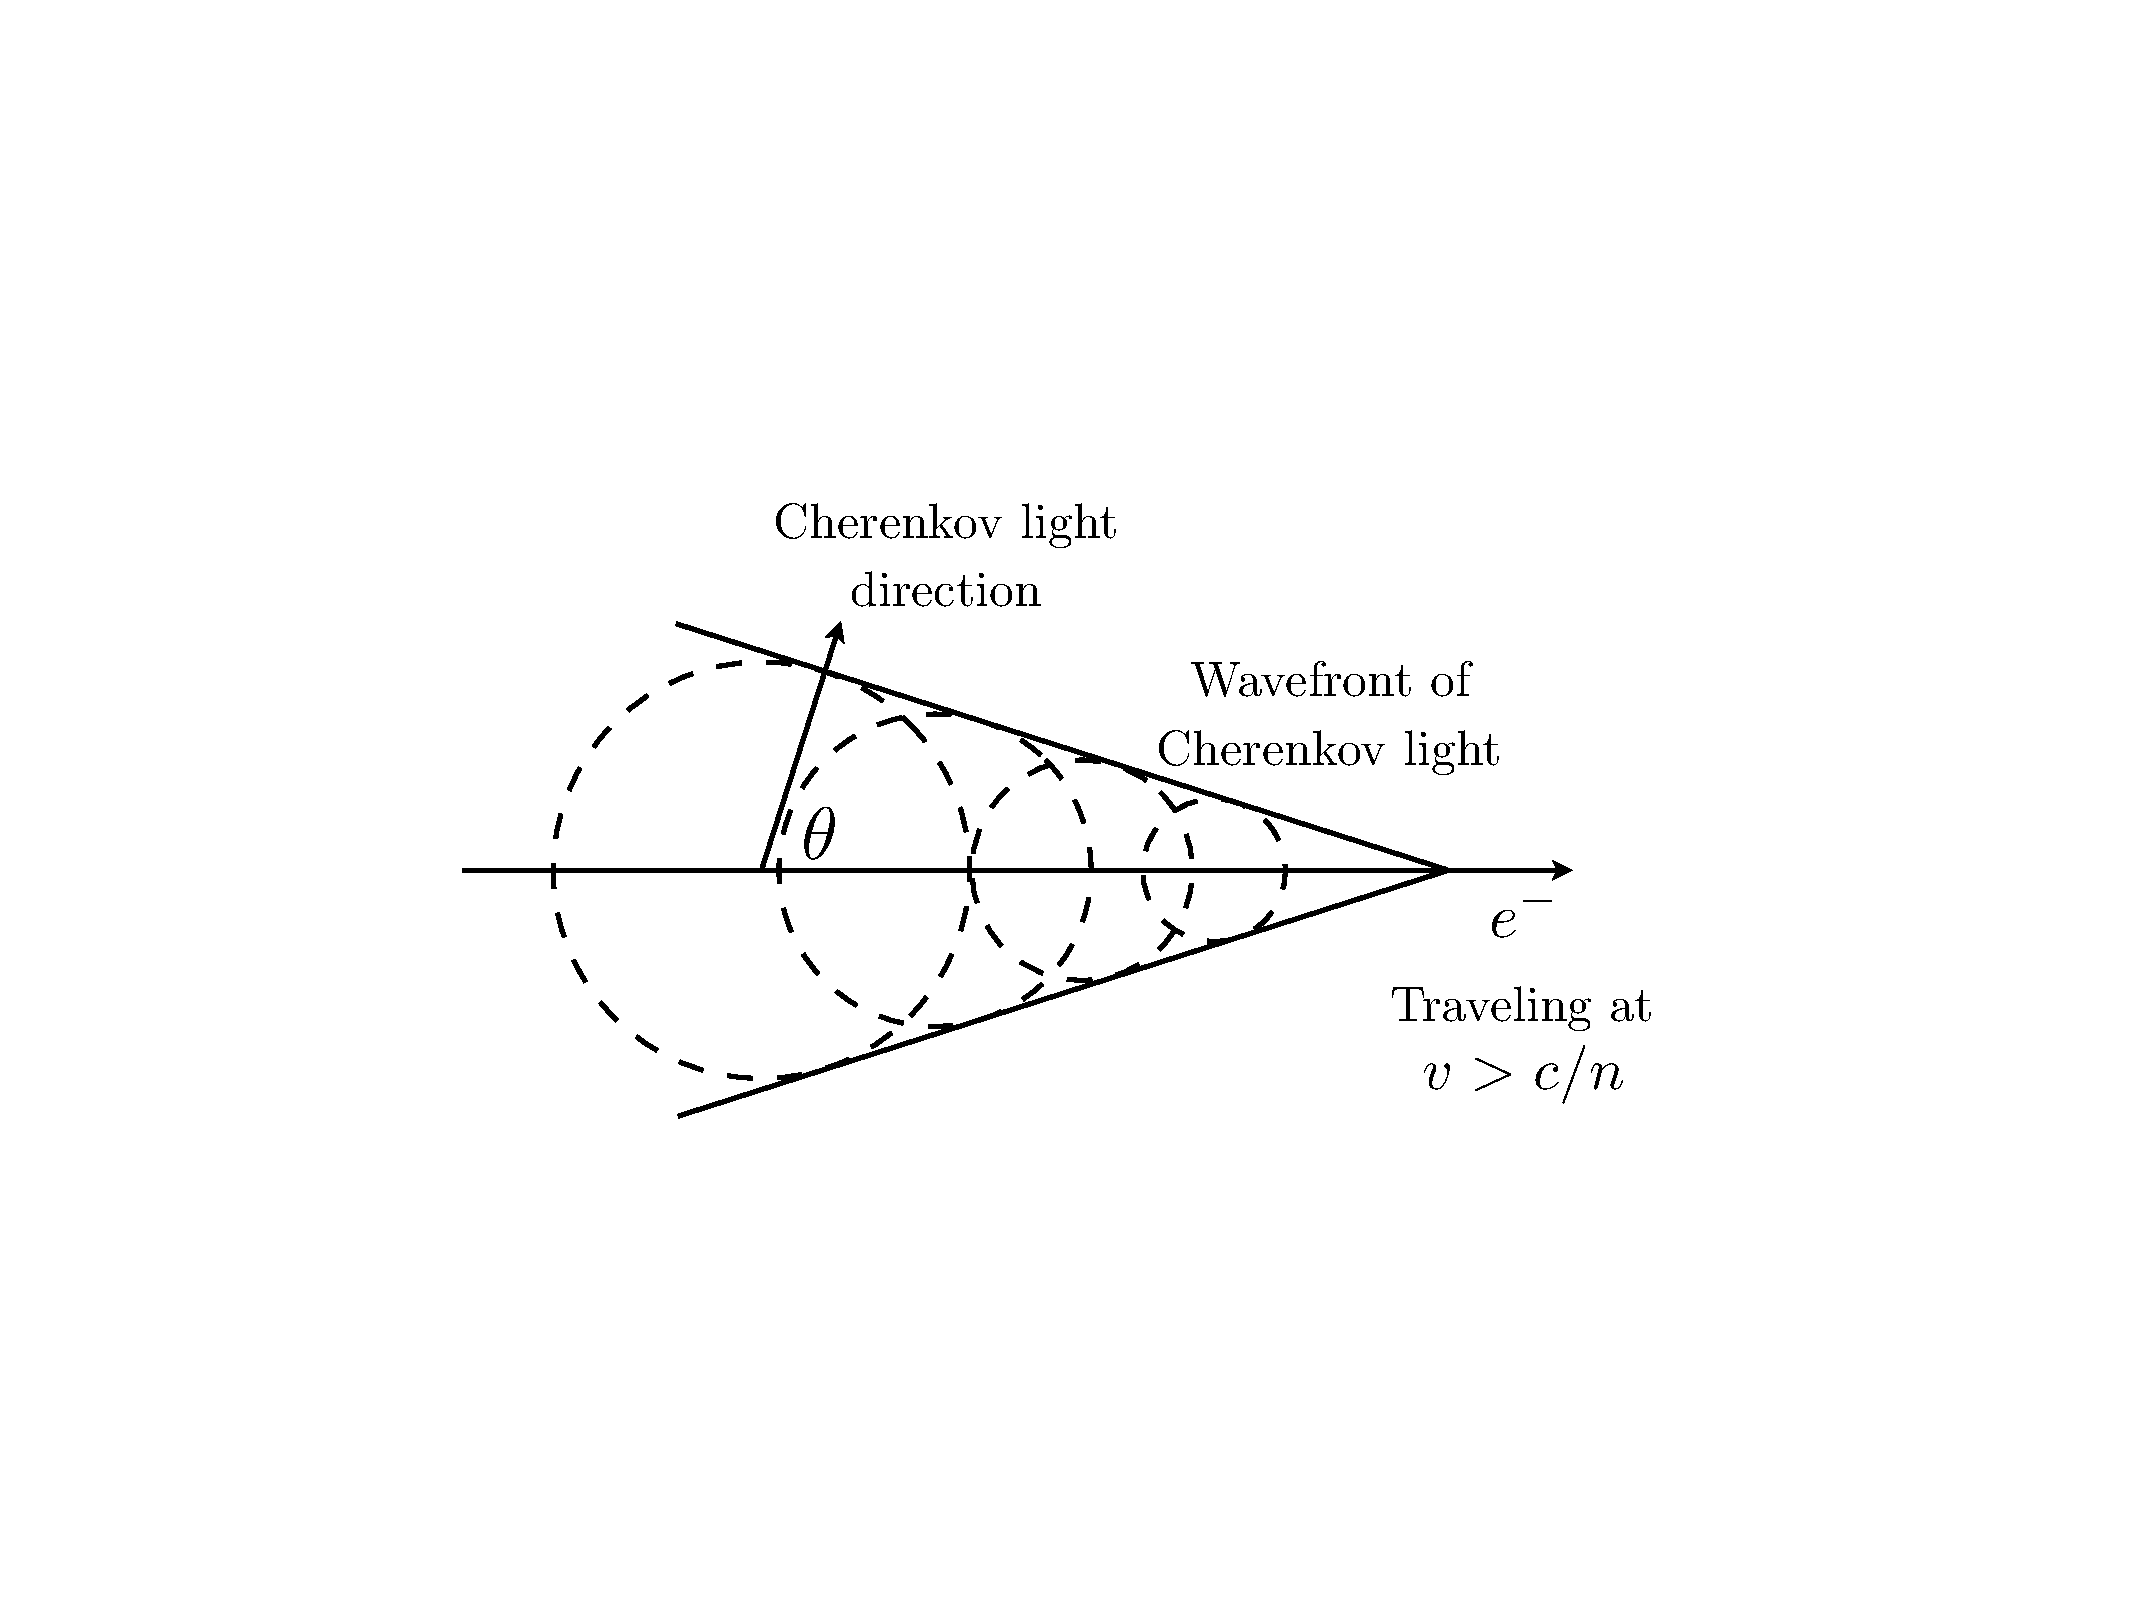
\includegraphics[width=0.6\textwidth]{figs/Cherenkov-radiation.pdf}
\caption[Cerenkov radiation]{The geometry of the emission of Cerenkov radiation.
\label{fig:Cerenkov-radiation}} 
\end{figure}

The threshold velocity and momentum for the production of Cerenkov light are given by:

\begin{equation} \label{Cerenkov_theshold_v}
\beta_{min} c = \frac{c}{n}
\end{equation}

\begin{equation} \label{Cerenkov_theshold_p}
p_{min} = \frac{mc}{\sqrt{n^2-1}}
\end{equation}

The threshold angle $\theta_c$ is given by: 

\begin{equation} \label{Cerenkov_direction}
\cos \theta_c = \frac{1}{\beta_{min} n}
\end{equation}

By detecting if a particle emit Cerenkov light, one can know if this particle's velocity is larger than threshold velocity
in the medium.


%with refraction index n, if the
%speed of particle $v = \beta c$ is higher than the speed of light $\frac{c}{n}$ in this medium,
%the particle will emit electromagnetic radiation called the Cerenkov light.
%Cerenkov light is emitted because the material becomes electrically polarized by the particle's electric field.
%If the speed of particle exceed the speed of light in the material, the 

During the CSR experiment the main background is pion. The Cerenkov detector can be used to separate 
electrons from pion background.
The gas Cerenkov detector is filled with CO$_2$ at atmospheric pressure.
With a refraction index n = 1.00041, the threshold momentum of electron and pion are:
\begin{equation} 
p_e = 17 \mathrm{MeV}/c, \;\; \mathrm{and} \;\;\;  p_{\pi} = 4.8 \mathrm{GeV}/c.
\end{equation}
Because the beam energy of CSR experiment range from 0.4 to to 4 GeV only electrons generate signals in the
Cerenkov and pions do not. The gas Cerenkov detector has an efficiency higher than 99\% in
identifying electrons.

The gas Cerenkov detector for each arm is installed between two scintillator planes, S1 and S2.
It is made of steel with thin entrance and exit window made of tedlar.
There are ten spherical mirrors installed as 5 (vertical) $\times$ 2(horizontal) arrray,
to focus the Cerenkov light on ten PMTs.
The mirrors have radius of curvature of 90 cm, and the PMTs are placed at $f=$90/2 = 45 cm from the mirrors,
such that parallel incident light can be focused on PMTs.
Signals from PMTs are sent to ADCs and summed together.
Even though pions cannot produce Cerenkov light, but they still can ionize the gas medium 
and thus generate secondary electrons. These secondary electrons may have high enough energy to trigger
Cerenkov detector and leave a background signal that lies near the single-photon-electron peak.
This background can be removed in the analysis using ADC cuts which will be explained in Chapter 4(Data Analysis).


\subsubsection{Electromagnetic Calorimeters}
The electromagnetic calorimeters provide an additional way of PID. When a high energy charged particle travels through 
lead glass, it will create a shower of photons and e$^-$/e$^+$ pairs. The photons created in this cascade process
will be collected by PMTs and the signal intensity is linearly proportional to the energy deposit of the incoming particle.
There will be two peaks in the output spectra, one peak with higher energy for electrons and another peak with lower energy
for pions. The double-layer configuration can provide PID because the second layer of lead glass calorimeter can further
separate electrons from contamination of pions.

The configurations of lead glass calorimeters on the LHRS and RHS are slightly different, see
Figure.~\ref{fig:calorimeters}.
The lead glass calorimeters on LHRS is composed of two layer of lead glass blocks with same geometry, each layer is called
a "pion rejector". Each layer consists of 17 long blocks and 17 short blocks, forming a 17(dispersive) $\times$
2(transverse) array, with dimension 14.5 cm $\times$ 14.5 cm $\times$ 30(or 35) cm.
Short blocks(30 cm long) and long blocks(35 cm long) are arranged interchangeablely in the dispersive direction for each row.

\begin{figure}[tb!]
\centering
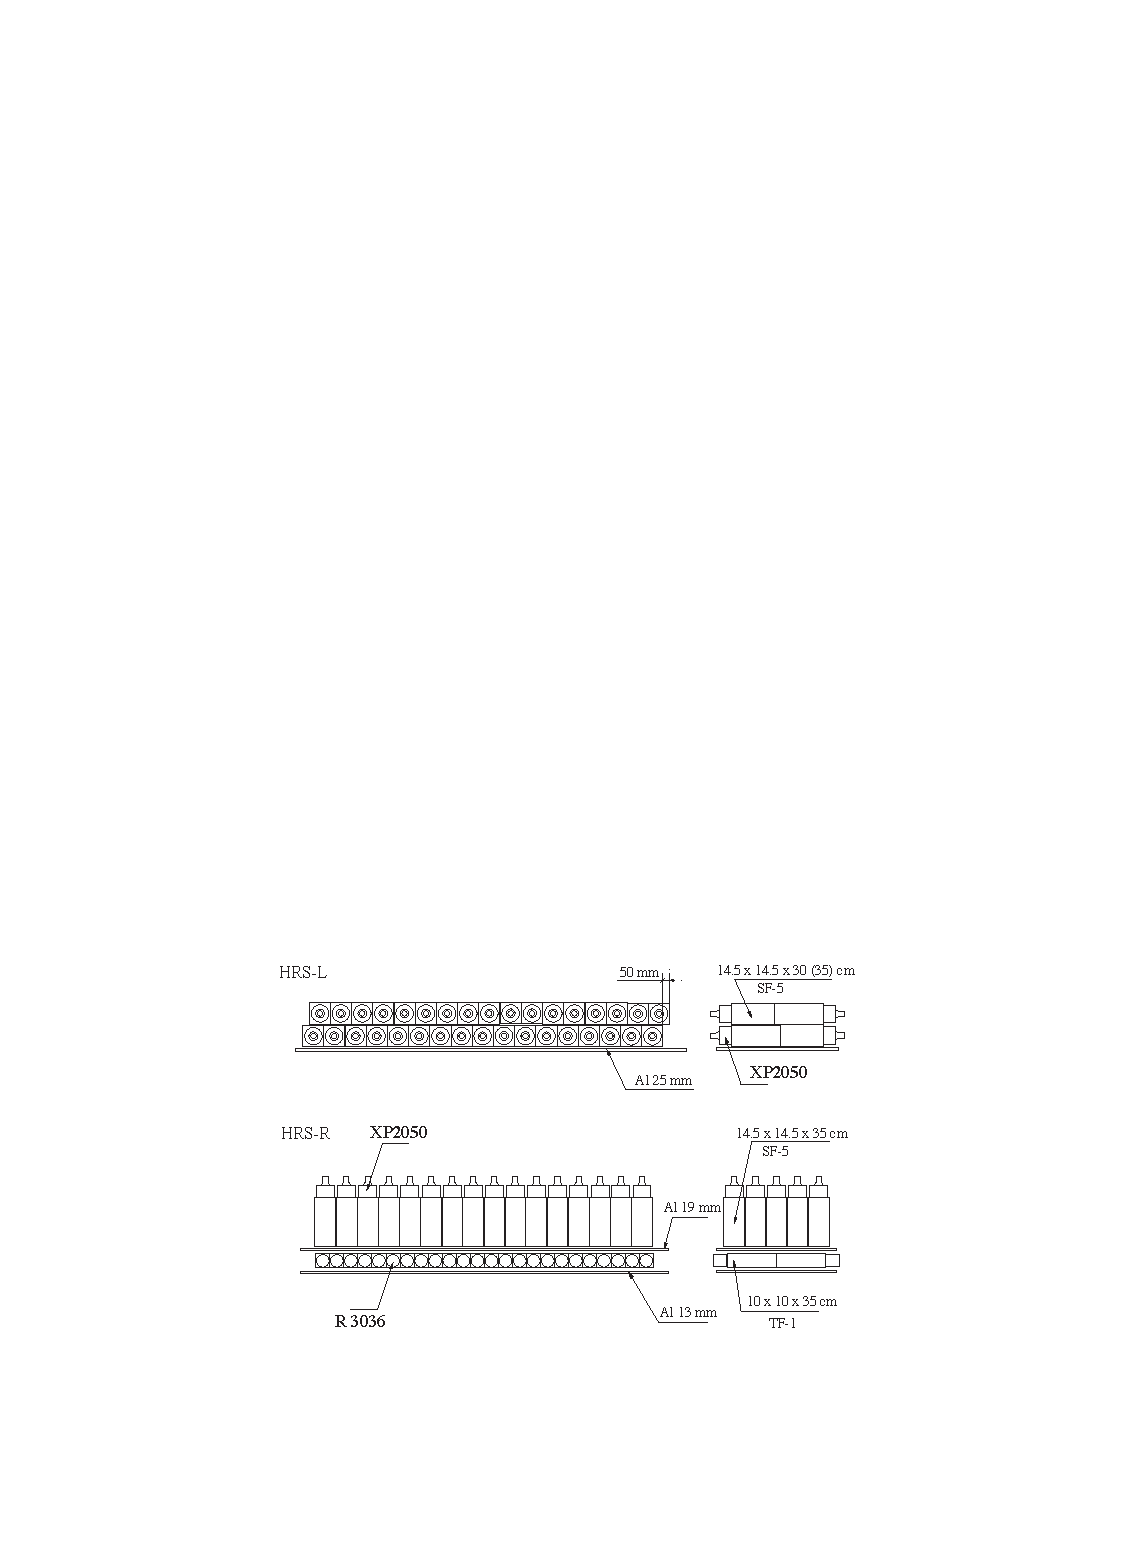
\includegraphics[width=0.8\textwidth]{figs/calorimeters.pdf}
\caption[Layout of electromagnetic calorimeters]{Schematic layout of electromagnetic calorimeters in left and right HRS.  \label{fig:calorimeters}}
\end{figure}

On the RHRS, the two layers are called "preshower" and "shower" respectively.
The first layer of lead glass blocks, "preshower", is arranged in an array of 24(dispersive) $\times$ 2 (transverse),
with dimension 35 cm $\times$ 10 cm $\times$ 10 cm, with the lead glass blocks perpendicular to the direction of
incoming electrons.
The "shower" is composed of 16(dispersive) $\times$ 5(transverse) blocks, with dimension 35 cm $\times$ 15 cm $\times$ 15 cm
which are oriented parallel to the electron trajectory.

The main difference between LHRS and RHRS lead-glass calorimeters is that the RHRS calorimeter is thick enough that 
electrons will deposit all their energies, while the calorimeter on LHRS is not a full energy absorber because of its
reduced thickness.


\section{Data Acquisition System}
The Data Acquisition system is used to collect event information from the detectors and beamline apparatus
and store the raw data.
The Hall A DAQ system is built on CEBAF Online Data Acquisition System (CODA), a software package specifically for
developed nuclear physics applications by the JLab data-acquisition group.  

CODA is composed of a set of software packages which can control DAQ hardwares such as front-end Fastbus VME digitization
devices (ADCs, TDCs, scalers), the VME Interface to Fastbus, single-board VME computers, and mass storage system(MSS).
%The custom software components of CODA are shown in Figure:
%A readout controller (ROC) runs on the front-end crates 
The raw data are divided into different runs for specific kinematics settings. Each run consists of several parts of
information:
\begin{itemize}
\item A header consists of information like run number, timestamp, event size and prescale factors.
\item CODA events which contain detectors and helicity information.
\item EPICS events contains information about beamline apparatus, spectrometer magnets setting and angle, target information
and other slow control device.
\item Scaler events which contain number of triggers and accumulated charges of the run.
\end{itemize}

\begin{figure}[tb!]
\centering
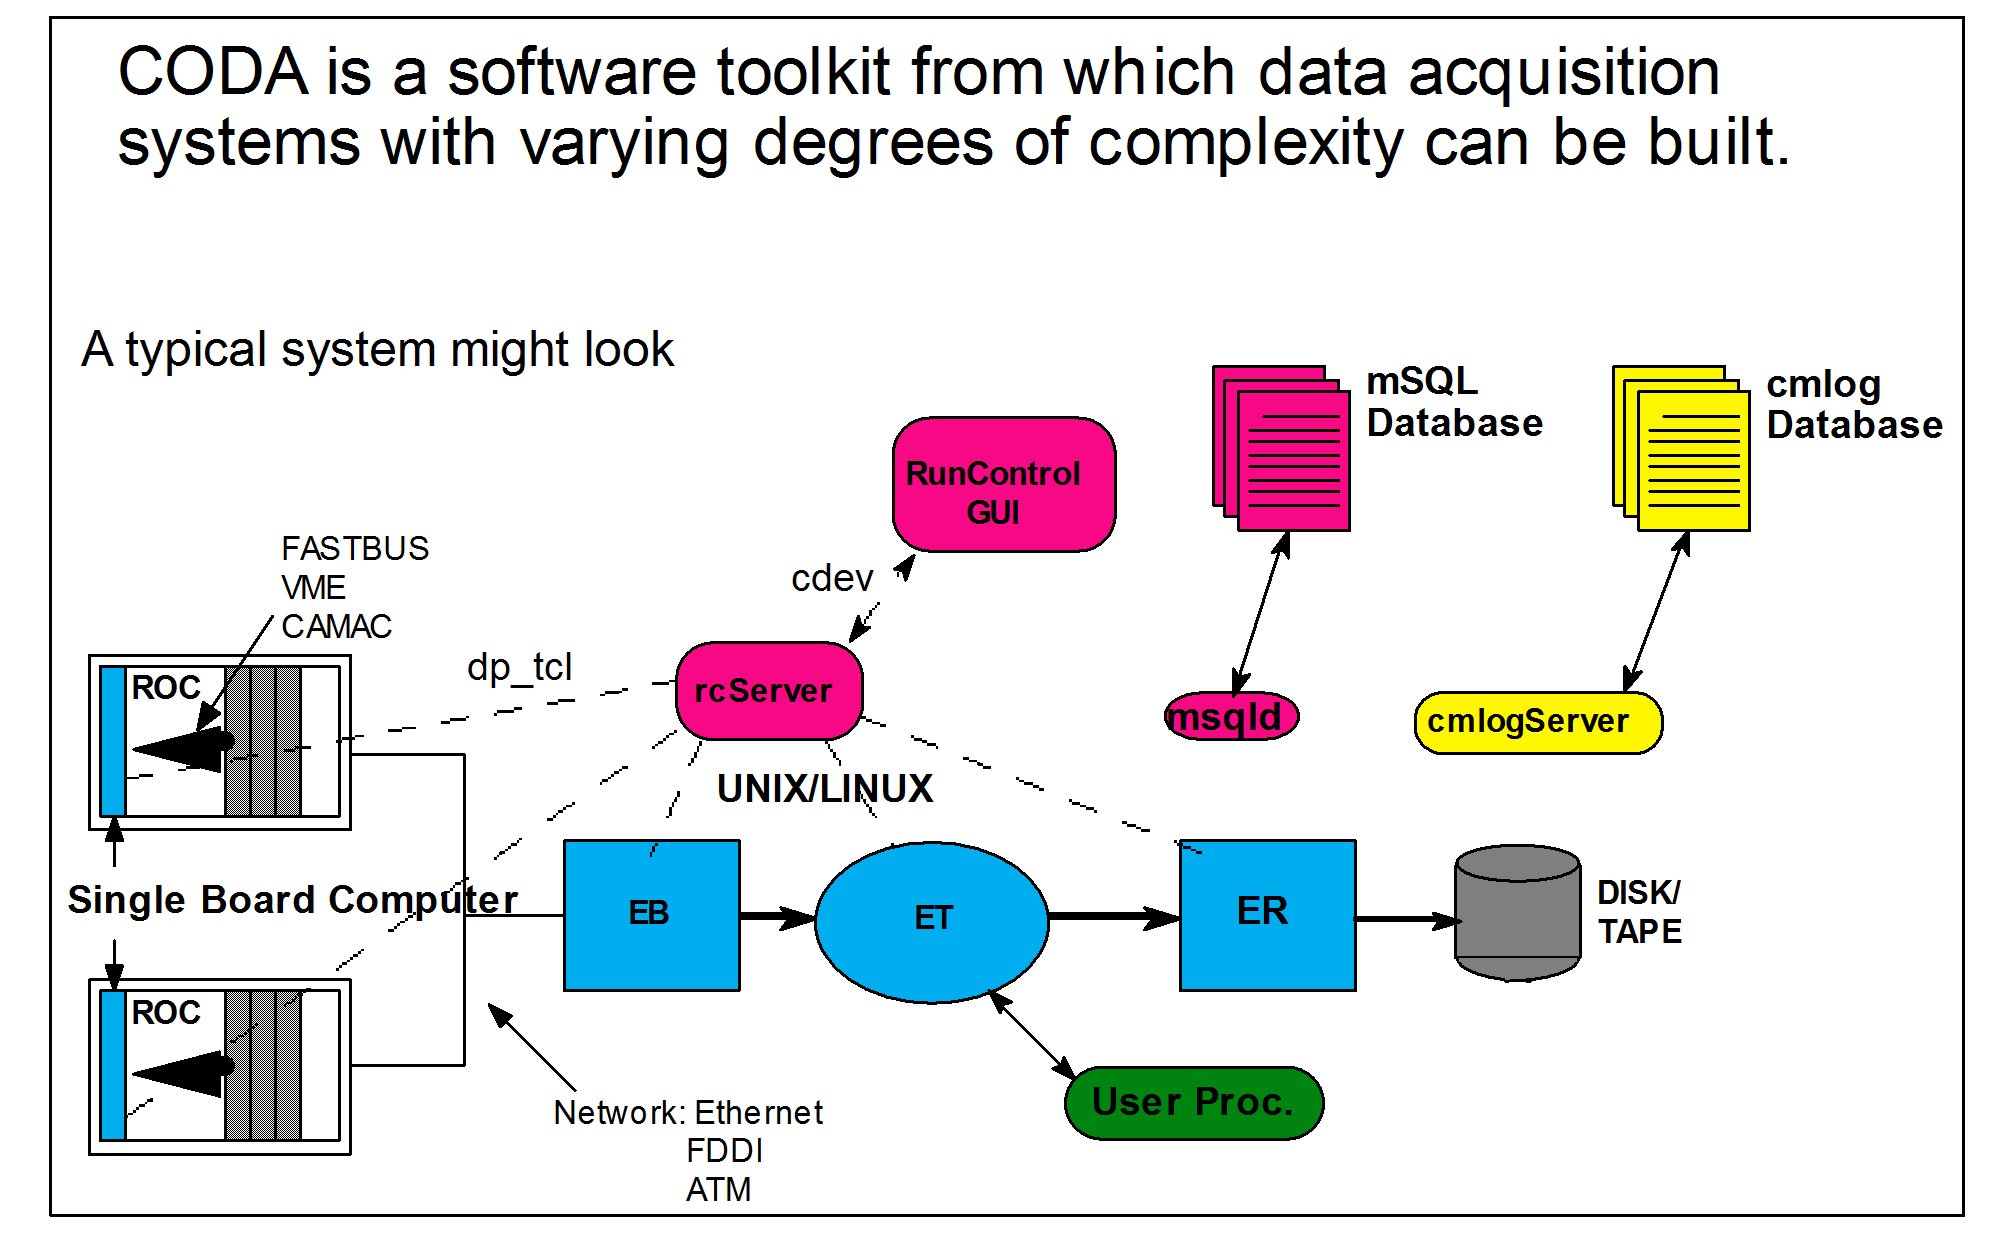
\includegraphics[width=0.8\textwidth]{figs/DAQ_diagram.png}
\caption[DAQ system diagram]{DAQ system diagram.  \label{fig:daq_diagram}}
\end{figure}

The data is first written to a local disk then moved to the Jefferson Lab Mass Storage System (MSS).
The total volume of data accumulated during the CSR experiment was about 3.0 TBytes.
%
%
%
%
%\cite{*}
%
%%%%%%%%%%%%%%%%%%%%%%%%%%%%%%%%%%%%%%%%%%%%%%%%%%%%%%%%%%%%%%%%%%%%%%%
%% -*-latex-*-
